\subsection{Künneth formula}

In this number, we consider a complex (C, d) of right A-modules and a complex (C', d') of left A-modules. Consider the canonical exact sequences

\[
0 \rightarrow \mathrm{Z} (\mathrm{C}) \stackrel {{j}} {{\rightarrow}} \mathrm{C} \stackrel {{\delta}} {{\rightarrow}} \mathrm{B} (\mathrm{C}) (- 1) \rightarrow 0,\tag{I}
\]

\[
0 \rightarrow \mathrm{B} (\mathrm{C}) \xrightarrow {i} \mathrm{Z} (\mathrm{C}) \xrightarrow {p} \mathrm{H} (\mathrm{C}) \rightarrow 0;\tag{II}
\]

we deduce from δ a k-homomorphism

\[
\mathrm{H} (\delta \otimes 1): \mathrm{H} (\mathrm{C} \otimes_ {\mathrm{A}} \mathrm{C} ^ {\prime}) \rightarrow \mathrm{H} (\mathrm{B} (\mathrm{C}) \otimes_ {\mathrm{A}} \mathrm{C} ^ {\prime}) (- 1);
\]

we deduce from (II) a connecting homomorphism

\[
\partial (\mathrm{II}, \mathrm{H} (\mathrm{C} ^ {\prime})): \operatorname{Tor} _ {1} ^ {\mathbf {A}} (\mathrm{H} (\mathrm{C}), \mathrm{H} (\mathrm{C} ^ {\prime})) \rightarrow \mathrm{B} (\mathrm{C}) \otimes_ {\mathbf {A}} \mathrm{H} (\mathrm{C} ^ {\prime});
\]

if we equip \(\operatorname{Tor}_{1}^{\mathbf{A}}(\mathrm{H}(\mathbf{C}),\mathrm{H}(\mathbf{C}^{\prime}))\) with the grading whose homogeneous component of degree \(n\) is \(\bigoplus_{p+q=n}\operatorname{Tor}_{1}^{\mathbf{A}}(\mathrm{H}_{p}(\mathbf{C}),\mathrm{H}_{q}(\mathbf{C}^{\prime}))\) , this connecting homomorphism is graded of degree 0. Moreover, there is a canonical homomorphism (X, p. 62)

\[
\gamma (\mathrm{B} (\mathrm{C}), \mathrm{C} ^ {\prime}): \mathrm{B} (\mathrm{C}) \otimes_ {\mathrm{A}} \mathrm{H} (\mathrm{C} ^ {\prime}) \rightarrow \mathrm{H} (\mathrm{B} (\mathrm{C}) \otimes_ {\mathrm{A}} \mathrm{C} ^ {\prime}).
\]

With these notations:

THEOREM 3. --- Suppose the A-modules B(C) and Z(C) are flat. There exists a unique homomorphism of graded k-modules, of degree -1,

\[
\alpha : \mathrm{H} (\mathrm{C} \otimes_ {\mathrm{A}} \mathrm{C} ^ {\prime}) \rightarrow \operatorname{Tor} _ {1} ^ {\mathrm{A}} (\mathrm{H} (\mathrm{C}), \mathrm{H} (\mathrm{C} ^ {\prime}))
\]

thereby making the diagram commutative

\[
\begin{array}{c} \mathrm{H} (\mathrm{C} \otimes_ {\mathrm{A}} \mathrm{C} ^ {\prime}) \xrightarrow {\alpha} \operatorname{Tor} _ {1} ^ {\mathrm{A}} (\mathrm{H} (\mathrm{C}), \mathrm{H} (\mathrm{C} ^ {\prime})) (- 1) \\ \mathrm{H} (\delta \otimes 1) \Biggl \downarrow \qquad \qquad \qquad \qquad \qquad \qquad \qquad \qquad \qquad \qquad \qquad \qquad \Biggl \downarrow \hat {c} (\Pi , \mathrm{H} (\mathrm{C} ^ {\prime})) \\ \mathrm{H} (\mathrm{B} (\mathrm{C}) \otimes_ {\mathrm{A}} \mathrm{C} ^ {\prime}) (- 1) \xleftarrow {\gamma (\mathrm{B} (\mathrm{C}) . \mathrm{C} ^ {\prime})} (\mathrm{B} (\mathrm{C}) \otimes_ {\mathrm{A}} \mathrm{H} (\mathrm{C} ^ {\prime})) (- 1). \end{array}
\]

The sequence of graded k-modules

\[
0 \longrightarrow \mathrm{H} (\mathrm{C}) \otimes_ {\mathrm{A}} \mathrm{H} \left(\mathrm{C} ^ {\prime}\right) \xrightarrow {\gamma \left(\mathrm{C} , \mathrm{C} ^ {\prime}\right)} \mathrm{H} \left(\mathrm{C} ^ {\prime} \otimes_ {\mathrm{A}} \mathrm{C} ^ {\prime}\right) \xrightarrow {\alpha} \operatorname{Tor} _ {1} ^ {\mathrm{A}} \left(\mathrm{H} (\mathrm{C}), \mathrm{H} \left(\mathrm{C} ^ {\prime}\right)\right) (- 1) \longrightarrow 0
\]

is exact.

Thus for each \( n \), we have an exact sequence

\[
\begin{array}{c} 0 \longrightarrow \bigoplus_ {p + q = n} \mathrm{H} _ {p} (\mathrm{C}) \otimes_ {\mathrm{A}} \mathrm{H} _ {q} (\mathrm{C} ^ {\prime}) \xrightarrow {\gamma_ {n} (\mathrm{C} , \mathrm{C} ^ {\prime})} \mathrm{H} _ {n} (\mathrm{C} \otimes_ {\mathrm{A}} \mathrm{C} ^ {\prime}) \\ \xrightarrow {\alpha_ {n}} \bigoplus_ {p + q = n - 1} \operatorname{Tor} _ {1} ^ {\mathrm{A}} \left(\mathrm{H} _ {p} (\mathrm{C}), \mathrm{H} _ {q} (\mathrm{C} ^ {\prime})\right) \longrightarrow 0. \end{array}\tag{11}
\]

For simplicity set \(\mathbf{B} = \mathbf{B}(\mathbf{C})\) , \(\mathbf{Z} = \mathbf{Z}(\mathbf{C})\) , \(\mathbf{H} = \mathbf{H}(\mathbf{C})\) and \(\mathbf{H}' = \mathbf{H}(\mathbf{C}')\) :

Since B is flat, we deduce from (I) an exact sequence (X, p. 72, cor. 2)

\[
0 \longrightarrow Z \otimes_ {A} C ^ {\prime} \xrightarrow {j \otimes 1} C \otimes_ {A} C ^ {\prime} \xrightarrow {\delta \otimes 1} (B \otimes_ {A} C ^ {\prime}) (- 1) \longrightarrow 0.\tag{12}
\]

Lemma 3. --- The connecting homomorphism H(B ⊗\_A C') → H(Z ⊗\_A C') associated with the exact sequence (12) is equal to H(i ⊗ 1).

Indeed, let \(a \in \mathbf{Z}(\mathbf{B} \otimes_{\mathbf{A}} \mathbf{C}')\) ; since B is flat, \(a\) belongs to the image of \(\mathbf{B} \otimes_{\mathbf{A}} \mathbf{Z}(\mathbf{C}')\) , hence can be written as \(\sum_{\lambda} da_{\lambda} \otimes b_{\lambda}\) , with \(a_{\lambda} \in \mathbf{C}\) , \(b_{\lambda} \in \mathbf{C}'\) , \(db_{\lambda} = 0\) . The image of

the class of \(a\) under the sought homomorphism is by definition the class of \(\mathbf{D}(\sum a_{\lambda}\otimes b_{\lambda})=\sum da_{\lambda}\otimes b_{\lambda}=(i\otimes1)(a)\) , whence the lemma.

The exact homology sequence associated with (12) is therefore

\[
\begin{array}{r l} \mathrm{H} (\mathrm{B} \otimes_ {\mathrm{A}} \mathrm{C} ^ {\prime}) & \xrightarrow {\mathrm{H} (i \otimes 1)} \mathrm{H} (\mathrm{Z} \otimes_ {\mathrm{A}} \mathrm{C} ^ {\prime}) \xrightarrow {\mathrm{H} (j \otimes 1)} \mathrm{H} (\mathrm{C} \otimes_ {\mathrm{A}} \mathrm{C} ^ {\prime}) \\ & \xrightarrow {\mathrm{H} (\delta \otimes 1)} \mathrm{H} (\mathrm{B} \otimes_ {\mathrm{A}} \mathrm{C} ^ {\prime}) (- 1) \xrightarrow {\mathrm{H} (i \otimes 1)} \mathrm{H} (\mathrm{Z} \otimes_ {\mathrm{A}} \mathrm{C} ^ {\prime}) (- 1). \end{array}
\]

Moreover, since Z is flat, we deduce from (II) an exact sequence of graded k-modules

\[
0 \longrightarrow \operatorname{Tor} _ {1} ^ {\mathrm{A}} (\mathrm{H}, \mathrm{H} ^ {\prime}) \xrightarrow {\hat {c} (\mathrm{II} , \mathrm{H} ^ {\prime})} \mathrm{B} \otimes_ {\mathrm{A}} \mathrm{H} ^ {\prime} \xrightarrow {i \otimes 1} Z \otimes_ {\mathrm{A}} \mathrm{H} ^ {\prime} \xrightarrow {p \otimes 1} \mathrm{H} \otimes_ {\mathrm{A}} \mathrm{H} ^ {\prime} \longrightarrow 0;
\]

finally, we have the canonical homomorphisms of no. 1

\[
\gamma_ {\mathbf {B}} = \gamma (\mathbf {B}, \mathbf {C} ^ {\prime}): \mathbf {B} \otimes_ {\mathbf {A}} \mathrm{H} ^ {\prime} \rightarrow \mathrm{H} (\mathbf {B} \otimes_ {\mathbf {A}} \mathbf {C} ^ {\prime})
\]

\[
\gamma_ {Z} = \gamma (Z, C ^ {\prime}): Z \otimes_ {A} H ^ {\prime} \rightarrow H (Z \otimes_ {A} C ^ {\prime})
\]

\[
\gamma_ {\mathrm{C}} = \gamma (\mathrm{C}, \mathrm{C} ^ {\prime}): \mathrm{H} \otimes_ {\mathrm{A}} \mathrm{H} ^ {\prime} \rightarrow \mathrm{H} (\mathrm{C} \otimes_ {\mathrm{A}} \mathrm{C} ^ {\prime}),
\]

whence a diagram of graded k-modules, with exact rows

\[
\begin{array}{r l} & \mathbf {B} \otimes \mathbf {H} ^ {\prime} \xrightarrow [ \gamma_ {B} ]{i \otimes 1} \mathbf {Z} \otimes \mathbf {H} ^ {\prime} \xrightarrow [ \gamma_ {Z} ]{p \otimes 1} \mathbf {H} \otimes \mathbf {H} ^ {\prime} \longrightarrow 0 \\ & \mathrm{H} (\mathbf {B} \otimes \mathbf {C} ^ {\prime}) \xrightarrow {\mathrm{H} (i \otimes 1)} \mathrm{H} (\mathbf {Z} \otimes \mathbf {C} ^ {\prime}) \xrightarrow {\mathrm{H} (j \otimes 1)} \mathrm{H} (\mathbf {C} \otimes \mathbf {C} ^ {\prime}) \xrightarrow {\mathrm{H} (\delta \otimes 1)} \mathrm{H} (\mathbf {B} \otimes \mathbf {C} ^ {\prime}) (- 1) \xrightarrow {\mathrm{H} (i \otimes 1)} \mathrm{H} (\mathbf {Z} \otimes \mathbf {C} ^ {\prime}) (- 1) \\ & 0 \longrightarrow \operatorname{Tor} _ {1} ^ {\mathrm{A}} (\mathrm{H}, \mathrm{H} ^ {\prime}) (- 1) \xrightarrow {\delta (\mathrm{II.H} ^ {\prime})} (\mathbf {B} \otimes \mathbf {H} ^ {\prime}) (- 1) \xrightarrow [ i \otimes 1 ]{\gamma_ {B}} (\mathbf {Z} \otimes \mathbf {H} ^ {\prime}) (- 1), \end{array}
\]

which is commutative by definition of homomorphisms \(\gamma\). But, since the complexes B and Z are split and flat, \(\gamma_{\mathbf{B}}\) and \(\gamma_{\mathbf{Z}}\) are bijective (X, p. 65, cor. 1). From this one deduces, on the one hand, that \(\gamma_{\mathbf{C}}\) is injective with image equal to Ker H( \(\delta \otimes 1\) ), and on the other hand that \(\gamma_{\mathbf{B}} \circ \partial(\mathrm{II}, \mathrm{H}')\) is injective, with image equal to Im H( \(\delta \otimes 1\) ). The theorem follows immediately from this.

COROLLARY 1. --- If B(C) and Z(C) are flat, then for every left A-module N and every integer n there is an exact sequence

\[
0 \longrightarrow \mathrm{H} _ {n} (\mathrm{C}) \otimes_ {\mathrm{A}} \mathrm{N} \xrightarrow {\gamma_ {n}} \mathrm{H} _ {n} (\mathrm{C} \otimes_ {\mathrm{A}} \mathrm{N}) \xrightarrow {\alpha_ {n}} \operatorname{Tor} _ {1} ^ {\mathrm{A}} \left(\mathrm{H} _ {n - 1} (\mathrm{C}), \mathrm{N}\right) \longrightarrow 0.\tag{13}
\]

COROLLARY 2. --- Suppose B(C) and B(C') are projective and Z(C) is flat. Then the sequences of k-modules (11) and (13) are exact and split.

This follows from the theorem and the following lemma:

Lemma 4. --- If B(C) and B(C') are projective, then the canonical homomorphism

\[
\gamma (\mathbf {C}, \mathbf {C} ^ {\prime}): \mathrm{H} (\mathbf {C}) \otimes_ {\mathbf {A}} \mathrm{H} (\mathbf {C} ^ {\prime}) \rightarrow \mathrm{H} (\mathbf {C} \otimes_ {\mathbf {A}} \mathbf {C} ^ {\prime})
\]

has a k-linear retraction.

Indeed, according to X, p. 65, remark b), there exist homologisms \(\varphi: C \to H(C)\) and \(\varphi': C' \to H(C')\) such that \(H(\varphi) = 1_{H(C)}\) and \(H(\varphi') = 1_{H(C')}\) . In the commutative diagram

\[
\begin{array}{c} \mathrm{H(C)} \otimes_ {\mathrm{A}} \mathrm {H(C^ {\prime})} \xrightarrow {\gamma (\mathrm{C,C} ^ {\prime})} \mathrm {H(C} \otimes_ {\mathrm{A}} \mathrm {C^ {\prime})} \\ \mathrm {H}(\varphi) \otimes \mathrm {H}(\varphi^ {\prime}) \Big \downarrow \\ \mathrm {H(C)} \otimes_ {\mathrm{A}} \mathrm {H(C^ {\prime})} \xrightarrow {\gamma (\mathrm{H(C),H(C^ {\prime})})} \mathrm {H(C)} \otimes_ {\mathrm{A}} \mathrm {H(C^ {\prime})} \end{array}
\]

\(\mathrm{H}(\varphi) \otimes \mathrm{H}(\varphi') \text{ and } \gamma(\mathrm{H}(\mathrm{C}), \mathrm{H}(\mathrm{C}') ) \text{ are the identity, whence the assertion.}\)

COROLLARY 3 (“universal coefficient formula”). --- Suppose the ring A is principal. If the complexes C and C' are free, then the sequences of A-modules (11) are exact and split; if the complex C is free, then the sequences of A-modules (13) are exact and split for every A-module N.

Indeed, B(C), Z(C), and B(C') are submodules of the free modules C, C, C', hence are free (VII, § 3, cor. 2 to th. 1), and one applies cor. 2.

COROLLARY 4 (“Künneth formula”). --- Suppose C is bounded above, and C and H(C) are flat; then the canonical homomorphism

\[
\gamma (\mathrm{C}, \mathrm{C} ^ {\prime}): \mathrm{H} (\mathrm{C}) \otimes_ {\mathrm{A}} \mathrm{H} (\mathrm{C} ^ {\prime}) \rightarrow \mathrm{H} (\mathrm{C} \otimes_ {\mathrm{A}} \mathrm{C} ^ {\prime})
\]

is bijective.

By the theorem, it suffices to prove that B(C) and Z(C) are flat. Now we have exact sequences

\[
0 \to \mathrm{B} _ {n} (\mathrm{C}) \to \mathrm{Z} _ {n} (\mathrm{C}) \to \mathrm{H} _ {n} (\mathrm{C}) \to 0
\]

\[
0 \to Z _ {n} (\mathbf {C}) \to \mathbf {C} _ {n} \to \mathbf {B} _ {n - 1} (\mathbf {C}) \to 0,
\]

whence, by X, p. 75, cor. 1, the implications \((\mathbf{B}_{n-1}(\mathbf{C})\) is flat) \(\Rightarrow (\mathbf{Z}_n(\mathbf{C})\) is flat) \(\Rightarrow (\mathbf{B}_n(\mathbf{C})\) is flat); we conclude by noting that \(\mathbf{B}_n(\mathbf{C}) = 0\) for \(n\) small enough.

COROLLARY 5. --- Let \(u: \mathbf{C} \to \mathbf{C}'\) a homomorphism of complexes of right A-modules, flat and bounded on the right. For every complex E of left A-modules, the morphism \(u \otimes 1_{\mathbf{E}}: \mathbf{C} \otimes_{\mathbf{A}} \mathbf{E} \to \mathbf{C}' \otimes_{\mathbf{A}} \mathbf{E}\) is a homologism.

Indeed, Con \((u)\) is a flat complex, bounded on the right and with zero homology; we therefore have H(Con \((u) \otimes_{\mathbf{A}} \mathbf{E}) = 0\) by cor. 4, hence H(Con \((u \otimes 1_{\mathbf{E}})) = 0\) (X, p. 67, lemma 2), and \(u \otimes 1_{\mathbf{E}}\) is a homologism.

\subsection{Bounded and flat complexes over a Noetherian ring}

PROPOSITION 11. --- Suppose A is left Noetherian, and let C be a bounded complex of flat left A-modules such that H(C) is a finitely generated A-module. Let a and b be two integers such that \(a \leqslant b\) and that \(\mathrm{H}_{n}(\mathrm{C}) = 0\) for \(n < a\) , \(\mathrm{C}_{n} = 0\) for \(n > b\) There exists a complex P of left A-modules such that \(\mathrm{P}_{n}\) is projective and finitely generated for each \(n\) , and that \(\mathrm{P}_{n} = 0\) for \(n \notin [a, b]\) , and a homologism \(u: \mathrm{P} \to \mathrm{C}\) . Moreover, for every complex E of right A-modules, the homomorphism

\[
\mathrm{H} \left(1 _ {\mathrm{E}} \otimes u\right): \mathrm{H} (\mathrm{E} \otimes_ {\mathrm{A}} \mathrm{P}) \rightarrow \mathrm{H} (\mathrm{E} \otimes_ {\mathrm{A}} \mathrm{C}) \quad \text{is bijective.}
\]

By X, p. 53, prop. 7, there exists a complex (L, d) such that \(L_{n}\) is free and finitely generated for each n, and zero when n \textless{} a, and a homologism \(f: L \to C\) . Let P be the quotient complex \(L/L'\) , where \(L_{n}' = 0\) for n \textless{} b, \(L_{n}' = L_{n}\) for n \textgreater{} b, \(L_{b}' = B_{b}(L)\) . Since \(C_{n} = 0\) for n \textgreater{} b, \(f(L') = 0\) , so f factors through a morphism of complexes \(u: P \to C\) .

\[
\begin{array}{c c c c c} \dots \longrightarrow & L _ {b + 1} & \xrightarrow {d _ {b + 1}} & L _ {b} & \xrightarrow {d _ {b}} L _ {b - 1} \longrightarrow \dots \\ & \downarrow & & \downarrow & | | \\ & 0 & \longrightarrow & P _ {b} & \longrightarrow P _ {b - 1} \longrightarrow \dots \\ & \downarrow & & \downarrow^ {u _ {b}} & \downarrow^ {u _ {b - 1}} \\ & 0 & \longrightarrow & C _ {b} & \longrightarrow C _ {b - 1} \longrightarrow \dots \end{array}
\]

Since \(f\) is a homologism, we have \(\mathrm{H}(\mathrm{Con}(f)) = 0\) whence an exact sequence

\[
\dots \rightarrow \mathrm{L} _ {b + 1} \xrightarrow {d _ {b + 1}} \mathrm{L} _ {b} \longrightarrow \mathrm{L} _ {b - 1} \oplus \mathrm{C} _ {b} \longrightarrow \mathrm{L} _ {b - 2} \oplus \mathrm{C} _ {b - 1} \rightarrow \dots .
\]

Thus we have an exact sequence

\[
0 \rightarrow \mathrm{P} _ {b} \rightarrow \mathrm{L} _ {b - 1} \oplus \mathrm{C} _ {b} \rightarrow \mathrm{L} _ {b - 2} \oplus \mathrm{C} _ {b - 1} \rightarrow \dots .
\]

This shows, on the one hand, that the cone of \(u\) has zero homology, so that \(u\) is a homologism, and on the other hand that the module \(\mathbf{P}_{b}\) is flat (X, p. 76, cor. 2); since \(\mathbf{P}_{b}\) is of finite type as a quotient of \(\mathbf{L}_{b+1}\) it is projective (X, p. 13, cor.). The pair (P, u) therefore satisfies the required condition. The last assertion follows from X, p. 79, cor. 5.

* Example. --- Let A be a Noetherian commutative ring, X a proper and flat A-scheme, \(\mathcal{F}\) a coherent \(\mathcal{O}_{\mathbf{X}}\)-module, flat over A. There exists a bounded complex P formed of finitely generated projective A-modules such that for every A-module M, H(X, \(\mathcal{F} \otimes_{\mathbf{A}} \mathbf{M}\) ) is naturally identified with H(P \(\otimes_{\mathbf{A}} \mathbf{M}\) ). Indeed, let \(\mathfrak{U}\) be a covering of X by a finite number of affine open sets, \(\mathcal{E}(\mathfrak{U}, \mathcal{F})\) the associated Čech complex: One shows that H \(^{i}\) ( \(\mathcal{E}(\mathfrak{U}, \mathcal{F})\) ) is isomorphic to the A-module H \(^{i}\) (X, \(\mathcal{F}\) ), and that the latter is finitely generated; moreover, for every A-module M, the complex \(\mathcal{E}(\mathfrak{U}, \mathcal{F}) \otimes_{\mathbf{A}} \mathbf{M}\) is isomorphic to \(\mathcal{E}(\mathfrak{U}, \mathcal{F} \otimes_{\mathbf{A}} \mathbf{M})\) . By applying prop. 11 to the complex \(\mathcal{E}(\mathfrak{U}, \mathcal{F})\) (which is bounded), one obtains a complex P which answers the question.

For every point \(y\) of \(\text{Spec}(\mathbf{A})\)  \(\kappa(y)\) the residue field of \(\mathbf{A}\) at \(y\) , \(X_y = X \otimes_{\mathbf{A}} \kappa(y)\) the fibre of \(\mathbf{X}\) above \(y\) , \(\mathcal{F}_y = \mathcal{F} \otimes_{\mathbf{A}} \kappa(y)\) , and set \(h^p(y) = \dim_{\kappa(y)} H^p(X_y, \mathcal{F}_y)\) for \(p \geqslant 0\) . One easily deduces from the existence of the complex \(\mathbf{P}\) the following results:

\begin{enumerate}
\def\labelenumi{(\roman{enumi})}
\item
  the function \(h^{p}\) is upper semi-continuous on Spec (A);
\item
  the function \(\sum_{p\geqslant 0}(-1)^{p}h^{p}\) is locally constant on \(\operatorname {Spec}(\mathbf{A})\) .*
\end{enumerate}

\subsection{Generalization to complexes of multimodules}

Let B and B' be two rings, C a complex of (B, A)-bimodules, C' a complex of (A, B')-bimodules (X, p. 43); then (C ⊗\_A C', D) (X, p. 61) is a complex of (B, B')-bimodules and the canonical homomorphism

\[
\gamma : \mathrm{H} (\mathbf {C}) \otimes_ {\mathbf {A}} \mathrm{H} (\mathbf {C} ^ {\prime}) \rightarrow \mathrm{H} (\mathbf {C} \otimes_ {\mathbf {A}} \mathbf {C} ^ {\prime})
\]

is compatible with the structures of (B, B')-bimodules of the two members.

If B'' is a third ring, and C'' a complex of (B', B'')-bimodules, the canonical homomorphism (II, p. 64, prop. 8)

\[
\left(\mathrm{C} \otimes_ {\mathrm{A}} \mathrm{C} ^ {\prime}\right) \otimes_ {\mathrm{B} ^ {\prime}} \mathrm{C} ^ {\prime \prime} \rightarrow \mathrm{C} \otimes_ {\mathrm{A}} \left(\mathrm{C} ^ {\prime} \otimes_ {\mathrm{B} ^ {\prime \prime}} \mathrm{C} ^ {\prime \prime}\right)
\]

is an isomorphism of complexes of (B, B'')-bimodules.

More generally, we leave it to the reader to develop the theory of tensor products of finite, totally ordered families of complexes of multimodules, following the model of no. 1 (X, p. 63) and of II, pp. 65 to 72 (associativity and commutativity isomorphisms, \ldots).

Let B and B′ be two rings, M a (B, A)-bimodule, N an (A, B′)-bimodule: then L(M) ⊗\_A L(N) is a complex of (B, B')-bimodules, so that Tor\^{}A (M, N) is endowed with a natural structure of graded (B, B')-bimodule; on the degree 0 term, this structure coincides with that of M ⊗\_A N.

If \(\lambda\in\mathbf{B},\lambda^{\prime}\in\mathbf{B}^{\prime}\) , and if we denote by \(\lambda_{\mathbf{M}},\lambda_{\mathbf{N}}^{\prime},\lambda_{\mathbf{T}},\lambda_{\mathbf{T}}^{\prime}\) , the homotheties \(x\mapsto\lambda x,y\mapsto y\lambda^{\prime},z\mapsto\lambda z,z\mapsto z\lambda^{\prime}\) of \(\mathbf{M},\mathbf{N},\mathrm{Tor}^{\mathbf{A}}(\mathbf{M},\mathbf{N}),\mathrm{Tor}^{\mathbf{A}}(\mathbf{M},\mathbf{N})\) respectively, then

\[
\lambda_ {\mathrm{T}} = \operatorname{Tor} ^ {\mathbf {A}} \left(\lambda_ {\mathbf {M}}, 1 _ {\mathbf {N}}\right), \quad \lambda_ {\mathrm{T}} ^ {\prime} = \operatorname{Tor} ^ {\mathbf {A}} \left(1 _ {\mathbf {M}}, \lambda_ {\mathbf {N}} ^ {\prime}\right),
\]

which provides another description of the bimodule structure of Tor \(^{A}\) (M, N). We leave it to the reader to generalize nos. 5 and 7 to the case of complexes of multimodules.

\section{EXTENSION MODULES}

We keep the general notation of § 4. We further agree that, unless expressly stated otherwise, all modules considered are left modules, and all complexes considered are complexes of left modules.

\subsection{Complexes of homomorphisms}

Let (C, d) and (C', d') be two A-complexes. Consider the graded k-module Homgr\_A (C, C') (II, pp. 174–175): for \(n \in \mathbf{Z}\) Homgr\_A (C, C')\_n is the k-module of graded A-linear maps of degree \(n\) from C to C'; in other words, Homgr\_A (C, C') is canonically identified with the A-module

\[
\bigoplus_ {n \in \mathbf {Z}} \prod_ {p \in \mathbf {Z}} \operatorname{Hom} _ {\mathrm{A}} \left(\mathrm{C} _ {p}, \mathrm{C} _ {p + n} ^ {\prime}\right) = \bigoplus_ {n \in \mathbf {Z}} \prod_ {p + q = n} \operatorname{Hom} _ {\mathrm{A}} \left(\mathrm{C} _ {p}, \mathrm{C} ^ {\prime q}\right).
\]

Let us define k-linear maps.

\[
\mathrm{D} _ {n}: \operatorname{Homgr} _ {\mathbf {A}} (\mathrm{C}, \mathrm{C} ^ {\prime}) _ {n} \rightarrow \operatorname{Homgr} _ {\mathbf {A}} (\mathrm{C}, \mathrm{C} ^ {\prime}) _ {n - 1}, \quad n \in \mathbf {Z},
\]

by

\[
\mathbf {D} _ {n} (f) = d ^ {\prime} \circ f - (- 1) ^ {n} f \circ d;\tag{1}
\]

we have

\[
\begin{array}{r l} \mathrm{D} _ {n - 1} \circ \mathrm{D} _ {n} (f) = & \mathrm{D} _ {n - 1} \left(d ^ {\prime} \circ f - (- 1) ^ {n} f \circ d\right) = d ^ {\prime} \circ d ^ {\prime} \circ f - (- 1) ^ {n} d ^ {\prime} \circ f \circ d \\ & - (- 1) ^ {n - 1} d ^ {\prime} \circ f \circ d - f \circ d \circ d = 0. \end{array}
\]

Then (Homgr \(_{A}\) (C, C'), D) is a complex of \(k\) -modules called the complex of homomorphisms from C to C'.

For example, \(\operatorname{Homgr}_{\mathbf{A}}(\mathbf{A}, \mathbf{C}')\) is canonically identified with \(\mathbf{C}'\). Let us also note that, for every \(n \in \mathbf{Z}\) , we have \(\operatorname{Homgr}_{\mathbf{A}}(\mathbf{C}, \mathbf{C}')\) ( \(n\) ) = \(\operatorname{Homgr}_{\mathbf{A}}(\mathbf{C}, \mathbf{C}'(n))\) .

The elements of \(Z_n(\text{Homgr}_A(C, C'))\) are the graded homomorphisms \(f\) of (descending) degree \(n\) of \(C\) to \(C'\) such that \(d' \circ f = (-1)^n f \circ d\) , that is, the morphisms of complexes of \(C\) to \(C'(n)\) , or again of \(C(p)\) to \(C'(p + n)\) for \(p\) any fixed. These are said to be the morphisms of complexes of (descending) degree \(n\) of \(C\) to \(C'\) ; if \(f, g \in Z_n(\text{Homgr}_A(C, C'))\) and \(s \in \text{Homgr}_A(C, C')_{n+1}\) , then the condition \(g - f = Ds\) means that \(s\) is a homotopy connecting the morphisms \(f\) and \(g\) of \(C\) to \(C'(n)\) , so that \(H_n(\text{Homgr}_A(C, C'))\) is the \(k\) -module of homotopy classes of morphisms of degree (descending) \(n\) of \(C\) to \(C'\) .

Let \(\alpha\in\mathrm{H}_{n}(\mathrm{Homgr}_{\mathrm{A}}(\mathrm{C},\mathrm{C}^{\prime}))\) and \(p\in\mathbf{Z}\) . Let us represent \(\alpha\) by \(f\in\mathbf{Z}_{n}(\mathrm{Homgr}_{\mathrm{A}}(\mathrm{C},\mathrm{C}^{\prime}))\) ; then \(f\) is a morphism of complexes of \(\mathbf{C}\) to \(\mathbf{C}^{\prime}(n)\) , hence \(\mathbf{H}_{p}(f)\) is a homomorphism of \(\mathbf{H}_{p}(\mathbf{C})\) to \(\mathbf{H}_{p}(\mathbf{C}^{\prime}(n))=\mathbf{H}_{p+n}(\mathbf{C}^{\prime})\) ; since \(\mathbf{H}_{p}(f)\) depends only on the homotopy class \(\alpha\) of \(f(\mathbf{X},\mathbf{p.~33,~prop.~3})\) , we deduce a canonical homomorphism of \(k\) -modules

\[
\mathrm{H} _ {n} \left(\operatorname{Homgr} _ {\mathrm{A}} \left(\mathrm{C}, \mathrm{C} ^ {\prime}\right)\right)\rightarrow \operatorname{Hom} _ {\mathrm{A}} \left(\mathrm{H} _ {p} (\mathrm{C}), \mathrm{H} _ {p + n} \left(\mathrm{C} ^ {\prime}\right)\right),
\]

whence a graded k-linear map of degree 0, called canonical

\[
\lambda (\mathrm{C}, \mathrm{C} ^ {\prime}): \mathrm{H} (\operatorname{Homgr} _ {\mathbf {A}} (\mathrm{C}, \mathrm{C} ^ {\prime})) \rightarrow \dot {\operatorname{Homgr}} _ {\mathbf {A}} (\mathrm{H} (\mathrm{C}), \mathrm{H} (\mathrm{C} ^ {\prime})).
\]

The homogeneous components of \(\lambda(C, C')\) will often be denoted:

\[
\lambda^ {n} (\mathrm{C}, \mathrm{C} ^ {\prime}): \mathrm{H} ^ {n} \left(\operatorname{Homgr} _ {\mathrm{A}} \left(\mathrm{C}, \mathrm{C} ^ {\prime}\right)\right)\rightarrow \prod_ {p + q = n} \operatorname{Hom} _ {\mathrm{A}} \left(\mathrm{H} _ {p} (\mathrm{C}), \mathrm{H} ^ {q} \left(\mathrm{C} ^ {\prime}\right)\right).
\]

PROPOSITION 1. --- If C is zero on the right and C' zero on the left, then Homgr \(_{A}\) (C, C') is zero on the left, and the canonical k-linear map

\[
\lambda^ {0} (\mathrm{C}, \mathrm{C} ^ {\prime}): \mathrm{H} ^ {0} \left(\operatorname{Homgr} _ {\mathrm{A}} (\mathrm{C}, \mathrm{C} ^ {\prime})\right)\rightarrow \operatorname{Hom} _ {\mathrm{A}} \left(\mathrm{H} _ {0} (\mathrm{C}), \mathrm{H} ^ {0} \left(\mathrm{C} ^ {\prime}\right)\right)
\]

is bijective.

We have exact sequences

\[
0 \longrightarrow \mathrm{H} ^ {0} (\mathrm{C} ^ {\prime}) \stackrel {i} {\longrightarrow} \mathrm{C} ^ {\prime 0} \stackrel {d ^ {\prime 0}} {\longrightarrow} \mathrm{C} ^ {\prime 1}
\]

\[
\mathrm{C} _ {1} \xrightarrow {d _ {1}} \mathrm{C} _ {0} \xrightarrow {p} \mathrm{H} _ {0} (\mathrm{C}) \longrightarrow 0.
\]

On the other hand \(\mathrm{Homgr}_{\mathbf{A}}^{0}(\mathbf{C},\mathbf{C}^{\prime})\) is identified with \(\mathrm{Hom}_{\mathbf{A}}(\mathbf{C}_{0},\mathbf{C}^{\prime 0})\) , \(\mathbf{Z}^{0}(\mathrm{Homgr}_{\mathbf{A}}(\mathbf{C},\mathbf{C}^{\prime}))\) then being identified with the set of \(f:\mathbf{C}_{0}\to \mathbf{C}^{\prime 0}\) such that \(d^{\prime 0}\circ f = 0\) , \(f\circ d_{1} = 0\) ; \(\mathbf{B}^{0}(\mathrm{Homgr}_{\mathbf{A}}(\mathbf{C},\mathbf{C}^{\prime}))\) is zero; finally the map \(\lambda^0\) associates to the class of \(f\) modulo \(\{0\}\) the homomorphism \(\varphi :\mathrm{H}_0(\mathrm{C})\to \mathrm{H}^0 (\mathrm{C}')\) such that \(f = i\circ \varphi \circ p\) , whence the proposition.

Let \(u: \tilde{\mathbf{C}} \to \mathbf{C}\) and \(u': \mathbf{C}' \to \tilde{\mathbf{C}}'\) be morphisms of complexes; then the canonical homomorphism \(\operatorname{Homgr}_{\mathbf{A}}(u, u') : \operatorname{Homgr}_{\mathbf{A}}(\mathbf{C}, \mathbf{C}') \to \operatorname{Homgr}_{\mathbf{A}}(\tilde{\mathbf{C}}, \tilde{\mathbf{C}}')\) , defined by \(f\mapsto u^{\prime}\circ f\circ u\) , is a morphism of complexes, as follows immediately from formula (1). Moreover, the following diagram is commutative

\[
\begin{array}{c} \mathrm{H} (\mathrm{Homgr} _ {\mathsf {A}} (\mathrm{C}, \mathrm{C} ^ {\prime})) \xrightarrow {\lambda (\mathrm{C} , \mathrm{C} ^ {\prime})} \mathrm{Homgr} _ {\mathsf {A}} (\mathrm{H} (\mathrm{C}), \mathrm{H} (\mathrm{C} ^ {\prime})) \\ \mathrm{H} (\mathrm{Homgr} _ {\mathsf {A}} (u, u ^ {\prime})) \Big \downarrow \\ \mathrm{H} (\mathrm{Homgr} _ {\mathsf {A}} (\tilde {\mathsf {C}}, \tilde {\mathsf {C}} ^ {\prime})) \xrightarrow {\lambda (\tilde {\mathsf {C}} , \tilde {\mathsf {C}} ^ {\prime})} \mathrm{Homgr} _ {\mathsf {A}} (\mathrm{H} (\tilde {\mathsf {C}}), \mathrm{H} (\tilde {\mathsf {C}} ^ {\prime}))  . \end{array}
\]

PROPOSITION 2. --- a) Let \(C' \xrightarrow{u} C \xrightarrow{v} C''\) be an exact sequence of A-complexes, \(P\) a projective complex, E an injective complex (X, p. 25). Then the sequences

\[
\operatorname{Homgr} _ {\mathbf {A}} (\mathrm{P}, \mathrm{C} ^ {\prime}) \xrightarrow {\operatorname{Homgr} (1 , u)} \operatorname{Homgr} _ {\mathbf {A}} (\mathrm{P}, \mathrm{C}) \xrightarrow {\operatorname{Homgr} (1 , v)} \operatorname{Homgr} _ {\mathbf {A}} (\mathrm{P}, \mathrm{C} ^ {\prime \prime})
\]

and

\[
\operatorname{Homgr} _ {\mathbf {A}} \left(\mathrm{C} ^ {\prime \prime}, \mathrm{E}\right) \xrightarrow {\operatorname{Homgr} (v , 1)} \operatorname{Homgr} _ {\mathbf {A}} (\mathrm{C}, \mathrm{E}) \xrightarrow {\operatorname{Homgr} (u , 1)} \operatorname{Homgr} _ {\mathbf {A}} \left(\mathrm{C} ^ {\prime}, \mathrm{E}\right)
\]

are exact sequences of complexes of k-modules.

\begin{enumerate}
\def\labelenumi{\alph{enumi})}
\setcounter{enumi}{1}
\tightlist
\item
  Let \(0 \to \mathbf{C}' \xrightarrow{u} \mathbf{C} \xrightarrow{v} \mathbf{C}'' \to 0\) be a sequence of A-complexes which is split as an exact sequence of graded A-modules (this is the case, for example, if \(\mathbf{C}'\) is injective, or if \(\mathbf{C}''\) is projective). Then for every complex E, the sequences
\end{enumerate}

\[
0 \rightarrow \operatorname{Homgr} _ {\mathbf {A}} (\mathrm{E}, \mathrm{C} ^ {\prime}) \xrightarrow {\operatorname{Homgr} (1 , u)} \operatorname{Homgr} _ {\mathbf {A}} (\mathrm{E}, \mathrm{C}) \xrightarrow {\operatorname{Homgr} (1 , v)} \operatorname{Homgr} _ {\mathbf {A}} (\mathrm{E}, \mathrm{C} ^ {\prime \prime}) \rightarrow 0
\]

\[
0 \rightarrow \operatorname{Homgr} _ {\mathbf {A}} \left(\mathrm{C} ^ {\prime \prime}, \mathrm{E}\right) \xrightarrow {\operatorname{Homgr} (v , 1)} \operatorname{Homgr} _ {\mathbf {A}} (\mathrm{C}, \mathrm{E}) \xrightarrow {\operatorname{Homgr} (u , 1)} \operatorname{Homgr} _ {\mathbf {A}} \left(\mathrm{C} ^ {\prime}, \mathrm{E}\right)\rightarrow 0
\]

are exact sequences of complexes of k-modules.

In the case \(a\) ), we note that the sequences

\[
\operatorname{Hom} _ {\mathbf {A}} \left(\mathrm{P} _ {p}, \mathrm{C} _ {q} ^ {\prime}\right)\rightarrow \operatorname{Hom} _ {\mathbf {A}} \left(\mathrm{P} _ {p}, \mathrm{C} _ {q}\right)\rightarrow \operatorname{Hom} _ {\mathbf {A}} \left(\mathrm{P} _ {p}, \mathrm{C} _ {q} ^ {\prime \prime}\right)
\]

and

\[
\operatorname{Hom} _ {\mathbf {A}} \left(\mathrm{C} _ {q} ^ {\prime \prime}, \mathrm{E} _ {p}\right)\rightarrow \operatorname{Hom} _ {\mathbf {A}} \left(\mathrm{C} _ {q}, \mathrm{E} _ {p}\right)\rightarrow \operatorname{Hom} _ {\mathbf {A}} \left(\mathrm{C} _ {q} ^ {\prime}, \mathrm{E} _ {p}\right)
\]

are exact for all \(p, q \in \mathbf{Z}\) , and we apply II, p. 10, prop. 5 and II, p. 13, prop. 7. The proof of \(b\) ) is analogous.

\subsection{Complexes of homomorphisms and homotopies}

PROPOSITION 3. --- Let C, \(\tilde{C}\) , \(C'\) , \(\tilde{C}'\) be four A-complexes, \(u: \tilde{C} \to C\) , \(v: \tilde{C} \to C\) , \(u': C' \to \tilde{C}'\) and \(v': C' \to \tilde{C}'\) four morphisms of complexes.

\begin{enumerate}
\def\labelenumi{\alph{enumi})}
\item
  If u and \(u'\) are homotopic to v and \(v'\) respectively, then the two morphisms \(\operatorname{Homgr}_{\mathbf{A}}(u, u')\) and \(\operatorname{Homgr}_{\mathbf{A}}(v, v')\) of \(\operatorname{Homgr}_{\mathbf{A}}(\mathbf{C}, \mathbf{C}')\) to \(\operatorname{Homgr}_{\mathbf{A}}(\tilde{\mathbf{C}}, \tilde{\mathbf{C}}')\) are homotopic.
\item
  If u and u' are homotopisms, Homgr\_A(u, u') is a homotopism.
\item
  If C or C' is homotopic to zero, Homgr\_A(C, C') is homotopic to zero.
\end{enumerate}

Let us denote by the same letter \(d\) the differentials of the complexes C, C \(_{1}\) , C \(^{\prime}\) , C \(_{1}^{\prime}\) , and by D the differentials of Homgr \(_{A}\) (C, C') and Homgr \(_{A}\) (C \(_{1}\) , C \(_{1}^{\prime}\) ). If \(u\) (resp. \(u^{\prime}\) ) is homotopic to \(v\) (resp. \(v^{\prime}\) ), there exists a graded homomorphism of degree 1,

\[
w: \mathrm{C} _ {1} \rightarrow \mathrm{C} \quad (\text { resp. } w ^ {\prime}: \mathrm{C} ^ {\prime} \rightarrow \mathrm{C} _ {1} ^ {\prime})
\]

such that

\[
u - v = d w + w d \quad (\text { resp. } u ^ {\prime} - v ^ {\prime} = d w ^ {\prime} + w ^ {\prime}\tag{2}
\]

Let W : Homgr \(_{A}\) (C, C') → Homgr \(_{A}\) (C \(_{1}\) , C \(_{1}\) ) be the graded homomorphism of degree 1 such that, for \(f \in\) Homgr \(_{A}\) (C, C') \(_{n}\) , \(n \in\) Z, we have

\[
\mathrm{W} (f) = w ^ {\prime} f u + (- 1) ^ {n} v ^ {\prime} f w.\tag{3}
\]

We then have

\[
\begin{array}{r l} (\mathrm{DW} + \mathrm{WD}) (f) & = \mathrm{D} [ w ^ {\prime} f u + (- 1) ^ {n} v ^ {\prime} f w ] + \mathrm{W} [ d f - (- 1) ^ {n} f d ] \\ & = d w ^ {\prime} f u - (- 1) ^ {n + 1} w ^ {\prime} f u d + (- 1) ^ {n} d v ^ {\prime} f w + v ^ {\prime} f w d \\ & \quad + w ^ {\prime} d f u + (- 1) ^ {n + 1} v ^ {\prime} d f w - (- 1) ^ {n} w ^ {\prime} f d u + v ^ {\prime} f d w \\ & = (d w ^ {\prime} + w ^ {\prime} d) f u + v ^ {\prime} f (w d + d w) \\ & = (u ^ {\prime} - v ^ {\prime}) f u + v ^ {\prime} f (u - v) = u ^ {\prime} f u - v ^ {\prime} f v; \end{array}
\]

which is written DW + WD = Homgr\_A (u, u')-Homgr\_A (v, v'), whence a).

Let us prove b). If u and \(u'\) are homotopisms, let \(\alpha: C \to \tilde{C}\) and \(\alpha': \tilde{C}' \to C'\) be morphisms of complexes such that \(u \circ \alpha\) , \(\alpha \circ u\) , \(u' \circ \alpha'\) , \(\alpha' \circ u'\) are homotopic respectively to \(Id_{C}\) , \(Id_{\tilde{C}}\) , \(Id_{\tilde{C}'}\) , \(Id_{C'}\) . Then Homgr \((u, u') \circ \text{Homgr } (\alpha, \alpha')\) , which is equal to Homgr \((\alpha \circ u, u' \circ \alpha')\) , is homotopic by a) to

\[
\operatorname{Homgr} _ {A} \left(\operatorname{Id} _ {C}, \operatorname{Id} _ {C ^ {\prime}}\right) = \operatorname{Id} _ {\operatorname{Homgr} (C, C ^ {\prime})}:
\]

likewise Homgr \((\alpha, \alpha') \circ\) Homgr \((u, u')\) is homotopic to \(\operatorname{Id}_{\operatorname{Homgr}(\tilde{\mathbb{C}}, \tilde{\mathbb{C}})}\) , whence \(b\) ).

Finally c) follows from b) (applied to the case where \(\tilde{C}\) or \(\tilde{C}'\) is zero).

COROLLARY 1. --- If C is split and H(C) is projective (resp. if C' is split and H \(_{n}\) (C') injective for each n), then the canonical homomorphism

\[
\lambda (\mathrm{C}, \mathrm{C} ^ {\prime}): \mathrm{H} (\operatorname{Homgr} _ {\mathrm{A}} (\mathrm{C}, \mathrm{C} ^ {\prime})) \rightarrow \operatorname{Homgr} _ {\mathrm{A}} (\mathrm{H} (\mathrm{C}), \mathrm{H} (\mathrm{C} ^ {\prime}))
\]

is bijective.

Suppose for example that C' is split and H(C') is injective for each n, the case where C is split and H(C) is projective being proved analogously. By X, p. 35, def. 6, there exists a homotopism \(u': C' \to H(C')\) ; by prop. 3, Homgr\_A (1, \(u'\) ) is a homotopism of Homgr\_A (C, C') on Homgr\_A (C, H(C')); since

\[
\operatorname{Homgr} _ {\mathbf {A}} \left(1, \mathrm{H} \left(u ^ {\prime}\right)\right) \circ \lambda (\mathrm{C}, \mathrm{C} ^ {\prime}) = \lambda (\mathrm{C}, \mathrm{H} \left(\mathrm{C} ^ {\prime}\right)) \circ \mathrm{H} \left(\operatorname{Homgr} _ {\mathbf {A}} \left(1, u ^ {\prime}\right)\right)
\]

and that \(\operatorname{Homgr}_{\mathbf{A}}(1, \mathrm{H}(u'))\) and \(\operatorname{H}(\operatorname{Homgr}_{\mathbf{A}}(1, u'))\) are bijective, it suffices for us to prove that \(\lambda(\mathbf{C},\mathbf{H}(\mathbf{C}^{\prime}))\) is bijective, which brings us back to the case where \(\mathbf{C}'\) is injective and has zero differential.

Then the canonical exact sequences (X, p. 28)

\[
0 \rightarrow \mathrm{B} (\mathrm{C}) \xrightarrow {i} \mathrm{C} \xrightarrow {p} \mathrm{C} / \mathrm{B} (\mathrm{C}) \rightarrow 0\tag{III}
\]

\[
0 \rightarrow \mathrm{H} (\mathrm{C}) \stackrel {{j}} {{\rightarrow}} \mathrm{C} / \mathrm{B} (\mathrm{C}) \stackrel {{\delta}} {{\rightarrow}} \mathrm{B} (\mathrm{C}) \rightarrow 0\tag{IV}
\]

give exact sequences (X, p. 83, prop. 2, a))

\[
0 \rightarrow \operatorname{Homgr} _ {\mathrm{A}} (\mathrm{C} / \mathrm{B} (\mathrm{C}), \mathrm{C} ^ {\prime}) \xrightarrow {\mathrm{P}} \operatorname{Homgr} _ {\mathrm{A}} (\mathrm{C}, \mathrm{C} ^ {\prime}) \xrightarrow {\mathrm{I}} \operatorname{Homgr} _ {\mathrm{A}} (\mathrm{B} (\mathrm{C}), \mathrm{C} ^ {\prime}) \rightarrow 0
\]

\[
0 \rightarrow \operatorname{Homgr} _ {\mathrm{A}} (\mathrm{B} (\mathrm{C}), \mathrm{C} ^ {\prime}) \stackrel {{\Delta}} {{\rightarrow}} \operatorname{Homgr} _ {\mathrm{A}} (\mathrm{C} / \mathrm{B} (\mathrm{C}), \mathrm{C} ^ {\prime}) \stackrel {{\mathrm{J}}} {{\rightarrow}} \operatorname{Homgr} _ {\mathrm{A}} (\mathrm{H} (\mathrm{C}), \mathrm{C} ^ {\prime}) \rightarrow 0.
\]

Since \(d_{\mathbf{C}} = i \circ \delta \circ p\) the differential D of Homgr(C, C') is given by \(\mathrm{D}_{n} = (-1)^{n+1} \mathrm{P}_{n} \circ \Delta_{n} \circ \mathrm{I}_{n}\) ; we then have

\[
\mathrm{Z} \left(\operatorname{Homgr} _ {\mathrm{A}} \left(\mathrm{C}, \mathrm{C} ^ {\prime}\right)\right) = \operatorname{Ker} (\mathrm{P} \circ \Delta \circ \mathrm{I}) = \operatorname{Ker} \mathrm{I} = \operatorname{Im} \mathrm{P},
\]

\[
\mathrm{B} \left(\operatorname{Homgr} _ {\mathrm{A}} \left(\mathrm{C}, \mathrm{C} ^ {\prime}\right)\right) = \operatorname{Im} (\mathrm{P} \circ \Delta \circ \mathrm{I}) = \mathrm{P} (\operatorname{Im} \Delta) = \mathrm{P} (\text { Ker   J });
\]

whence an isomorphism \(\varphi : H(\text{Homgr}_A(C, C')) \to \text{Homgr}_A(H(C), C')\) such that, if \(a \in \text{Homgr}_A(C/B(C), C')\) , then the image under \(\varphi\) of the class of \(P(a)\) is \(J(a)\) ; one immediately verifies that \(\varphi\) identifies with the canonical homomorphism \(\lambda\) .

COROLLARY 2. --- Suppose B(C) and H(C) are projective (resp. B \(_{n}\) (C') and H \(_{n}\) (C') injective for each n). Then λ(C, C') is bijective.

Indeed C (resp. C′) is then split by X, p. 35, example 4, and we apply Cor. 1.

COROLLARY 3. --- Let M be a projective (resp. injective) A-module. For every complex C of A-modules and every integer n, the canonical homomorphism

\[
\mathrm{H} ^ {n} (\operatorname{Homgr} _ {\mathbf {A}} (\mathrm{M}, \mathrm{C})) \rightarrow \operatorname{Hom} _ {\mathbf {A}} (\mathrm{M}, \mathrm{H} ^ {n} (\mathrm{C}))
\]

\[
\left(\text { resp. } \mathrm{H} ^ {n} (\operatorname{Homgr} _ {\mathbf {A}} (\mathbf {C}, \mathbf {M})) \rightarrow \operatorname{Hom} _ {\mathbf {A}} \left(\mathrm{H} _ {n} (\mathbf {C}), \mathbf {M}\right)\right) \text { is   bijective. }
\]

Lemma 1. --- a) If C or C′ is bounded on the right, if C is projective and if H(C′) = 0, then H(Homgr\_A(C, C')) = 0.

\begin{enumerate}
\def\labelenumi{\alph{enumi})}
\setcounter{enumi}{1}
\tightlist
\item
  If C or C' is bounded on the left, if C' is injective and if H(C) = 0, then H(Homgr\_A(C, C')) = 0.
\end{enumerate}

Let \(f \in Z_n(\text{Homgr}_A(C, C'))\) ; \(f\) is therefore a morphism of complexes of \(C\) to \(C'(n)\) ; in the case \(a\) (resp. \(b\) ), \(f_m\) is zero for \(m\) small enough (resp. large enough). By \(X\) , p. 47, prop. 1, \(f\) is then homotopic to zero, hence belongs to \(B_n(\text{Homgr}_A(C, C'))\) whence the conclusion.

PROPOSITION 4. --- Let \(u: \mathbb{C}' \to \mathbb{C}\) be a homologism of complexes, \(\mathbb{P}\) a projective complex, \(\mathbb{E}\) an injective complex.

\begin{enumerate}
\def\labelenumi{\alph{enumi})}
\tightlist
\item
  If P is bounded above, or if C and C' are bounded above, then
\end{enumerate}

\[
\operatorname{Homgr} _ {\mathbf {A}} (1, u): \operatorname{Homgr} _ {\mathbf {A}} (\mathrm{P}, \mathrm{C} ^ {\prime}) \rightarrow \operatorname{Homgr} _ {\mathbf {A}} (\mathrm{P}, \mathrm{C})
\]

is a homologism.

\begin{enumerate}
\def\labelenumi{\alph{enumi})}
\setcounter{enumi}{1}
\tightlist
\item
  If E is bounded below, or if C and C' are bounded below, then
\end{enumerate}

\[
\operatorname{Homgr} _ {\mathbf {A}} (u, 1): \operatorname{Homgr} _ {\mathbf {A}} (\mathrm{C}, \mathrm{E}) \rightarrow \operatorname{Homgr} _ {\mathbf {A}} (\mathrm{C} ^ {\prime}, \mathrm{E})
\]

is a homologism.

Suppose first that u is injective, and set \(C'' = \text{Coker } u\) . Since u is a homologism, \(C''\) has zero homology. On the other hand, we have exact sequences (prop. 2)

\[
0 \rightarrow \operatorname{Homgr} _ {\mathrm{A}} (\mathrm{P}, \mathrm{C} ^ {\prime}) \xrightarrow {\operatorname{Homgr} (1 , u)} \operatorname{Homgr} _ {\mathrm{A}} (\mathrm{P}, \mathrm{C}) \rightarrow \operatorname{Homgr} _ {\mathrm{A}} (\mathrm{P}, \mathrm{C} ^ {\prime \prime}) \rightarrow 0
\]

\[
0 \rightarrow \operatorname{Homgr} _ {\mathbf {A}} \left(\mathrm{C} ^ {\prime \prime}, \mathrm{E}\right)\rightarrow \operatorname{Homgr} _ {\mathbf {A}} (\mathrm{C}, \mathrm{E}) \xrightarrow {\operatorname{Homgr} (u , 1)} \operatorname{Homgr} _ {\mathbf {A}} \left(\mathrm{C} ^ {\prime}, \mathrm{E}\right)\rightarrow 0
\]

by lemma 1, Homgr \(_{A}\) (P, C'') has zero homology in the case \(a\) ), Homgr \(_{A}\) (C'', E) has zero homology in the case \(b\) ), whence the conclusion.

In the general case, there exists (X, p. 38, cor. to prop. 7) a complex \(\tilde{\mathbf{C}}'\) , which is bounded on the right (resp. on the left) when C and C' are, an injective morphism \(\tilde{u}: \mathbf{C}' \to \tilde{\mathbf{C}}'\) and a homotopism \(\beta: \tilde{\mathbf{C}}' \to \mathbf{C}\) such that \(u = \beta \circ \tilde{u}\) . Then \(\tilde{u}\) is a homologism (X, p. 34, cor. to prop. 5); by the preceding, Homgr \(_{\mathbf{A}}\) ( \(1_{\mathbf{P}}, \tilde{u}\) ) (resp. Homgr \(_{\mathbf{A}}\) ( \(\tilde{u}, 1_{\mathbf{E}}\) )) is a homologism in the case \(a\) ) (resp. \(b\) ). On the other hand Homgr \(_{\mathbf{A}}\) ( \(1_{\mathbf{P}}, \beta\) ) (resp. Homgr \(_{\mathbf{A}}\) ( \(\beta, 1_{\mathbf{E}}\) )) is a homotopism (prop. 3): then Homgr \(_{\mathbf{A}}\) ( \(1_{\mathbf{P}}, u\) ) (resp. Homgr \(_{\mathbf{A}}\) ( \(u, 1_{\mathbf{E}}\) )) is composed of two homologisms, hence is a homologism.

\subsection{Definition and first properties of extension modules}

For every A-module E, we denote by \(p_{\mathbf{E}} : \mathbf{L}(\mathbf{E}) \to \mathbf{E}\) (resp. \(e_{\mathbf{E}} : \mathbf{E} \to \mathbf{I}(\mathbf{E})\) ) the canonical free (resp. injective) resolution, cf. X, p. 50 (resp. p. 52).

DEFINITION 1. --- Let M and N be two A-modules. One calls the extension module of N by M the graded k-module

\[
\operatorname{Ext} _ {\mathbf {A}} (\mathbf {M}, \mathbf {N}) = \mathrm{H} \left(\operatorname{Homgr} _ {\mathbf {A}} (\mathrm{L} (\mathbf {M}), \mathrm{I} (\mathbf {N}))\right).\tag{4}
\]

The homogeneous components of Ext \(_{A}\) (M, N) are denoted

\[
\operatorname{Ext} _ {\mathbf {A}} ^ {n} (\mathbf {M}, \mathbf {N}) = \mathrm{H} ^ {n} \left(\operatorname{Homgr} _ {\mathbf {A}} (\mathbf {L} (\mathbf {M}), \mathrm{I} (\mathbf {N}))\right).\tag{5}
\]

Since L(M) (resp. I(N)) is zero on the right (resp. left), we have

\[
\operatorname{Ext} _ {\mathbf {A}} ^ {n} (\mathbf {M}, \mathbf {N}) = 0 \quad \text { for } \quad n <   0.\tag{6}
\]

Remark 1. --- We shall see below (X, p. 107, prop. 6) finiteness properties of the modules Ext \(_{A}\) (M, N). For example, if A is commutative Noetherian, and if M and N are finitely generated A-modules, each A-module Ext \(_{A}^{n}\) (M, N) is finitely generated.

Let \(f: \mathbf{M}' \to \mathbf{M}\) and \(g: \mathbf{N} \to \mathbf{N}'\) homomorphisms of A-modules, we set

\[
\operatorname{Ext} _ {\mathbf {A}} (f, g) = \mathrm{H} \left(\operatorname{Homgr} _ {\mathbf {A}} (\mathrm{L} (f), \mathrm{I} (g))\right);
\]

it is a degree 0 homomorphism of graded k-modules

\[
\operatorname{Ext} _ {\mathbf {A}} (f, g): \operatorname{Ext} _ {\mathbf {A}} (\mathbf {M}, \mathbf {N}) \rightarrow \operatorname{Ext} _ {\mathbf {A}} \left(\mathbf {M} ^ {\prime}, \mathbf {N} ^ {\prime}\right),
\]

whose homogeneous components are denoted

\[
\operatorname{Ext} _ {\mathbf {A}} ^ {n} (f, g): \operatorname{Ext} _ {\mathbf {A}} ^ {n} (\mathbf {M}, \mathbf {N}) \rightarrow \operatorname{Ext} _ {\mathbf {A}} ^ {n} \left(\mathbf {M} ^ {\prime}, \mathbf {N} ^ {\prime}\right).
\]

By prop. 1 of X, p. 82, the canonical homomorphism

\[
\lambda^ {0} (\mathrm{L} (\mathrm{M}), \mathrm{I} (\mathrm{N})): \mathrm{H} ^ {0} \left(\operatorname{Homgr} _ {\mathrm{A}} (\mathrm{L} (\mathrm{M}), \mathrm{I} (\mathrm{N}))\right)\rightarrow \operatorname{Hom} _ {\mathrm{A}} \left(\mathrm{H} _ {0} (\mathrm{L} (\mathrm{M})), \mathrm{H} ^ {0} (\mathrm{I} (\mathrm{N}))\right)
\]

is bijective; using the isomorphisms \(\mathbf{M} \to \mathrm{H}_{0}(\mathrm{L}(\mathbf{M}))\) and \(\mathrm{H}^{0}(\mathrm{I}(\mathbf{N})) \to \mathbf{N}\) , we deduce an isomorphism said to be canonical

\[
\lambda_ {\mathbf {M}, \mathbf {N}}: \operatorname{Ext} _ {\mathbf {A}} ^ {0} (\mathbf {M}, \mathbf {N}) \rightarrow \operatorname{Hom} _ {\mathbf {A}} (\mathbf {M}, \mathbf {N}).\tag{7}
\]

One will always identify \(\operatorname{Ext}_{\mathbf{A}}^{0}(\mathbf{M},\mathbf{N})\) with \(\operatorname{Hom}_{\mathbf{A}}(\mathbf{M},\mathbf{N})\) by this isomorphism. Then the map \(k\) -linear \(\operatorname{Ext}_{\mathbf{A}}^{0}(f,g)\) is identified with \(\operatorname{Hom}_{\mathbf{A}}(f,g)\) .

Remark 2. --- The morphism of complexes

\[
\operatorname{Homgr} _ {\mathbf {A}} \left(p _ {\mathbf {M}}, e _ {\mathbf {N}}\right): \operatorname{Hom} _ {\mathbf {A}} (\mathbf {M}, \mathbf {N}) \rightarrow \operatorname{Homgr} _ {\mathbf {A}} \left(\mathbf {L} (\mathbf {M}), \mathrm{I} (\mathbf {N})\right)
\]

induces on the homology of degree 0 the isomorphism

\[
\lambda_ {\mathbf {M}, \mathbf {N}} ^ {- 1}: \operatorname{Hom} _ {\mathbf {A}} (\mathbf {M}, \mathbf {N}) \rightarrow \operatorname{Ext} _ {\mathbf {A}} ^ {0} (\mathbf {M}, \mathbf {N})
\]

inverse of \(\lambda_{M,N}\) .

One has \(L(1_{\mathbf{M}}) = 1_{L(\mathbf{M})}\) , \(I(1_{\mathbf{N}}) = 1_{I(\mathbf{N})}\) , hence by passing to homology

\[
\operatorname{Ext} _ {\mathbf {A}} \left(1 _ {\mathbf {M}}, 1 _ {\mathbf {N}}\right) = 1 _ {\operatorname{Ext} _ {\mathbf {A}} (\mathbf {M}, \mathbf {N})}.\tag{8}
\]

If \(f': M'' \to M'\) and \(g': N' \to N''\) are homomorphisms of A-modules, we have \(L(f \circ f') = L(f) \circ L(f')\) and \(I(g' \circ g) = I(g') \circ I(g)\) , hence

\[
\operatorname{Ext} _ {\mathbf {A}} \left(f \circ f ^ {\prime}, g ^ {\prime} \circ g\right) = \operatorname{Ext} _ {\mathbf {A}} \left(f ^ {\prime}, g ^ {\prime}\right) \circ \operatorname{Ext} _ {\mathbf {A}} (f, g).\tag{9}
\]

Consider the morphisms of k-complexes

\[
\operatorname{Homgr} _ {\mathbf {A}} (\mathrm{L} (\mathrm{M}), \mathrm{N}) \xrightarrow {\operatorname{Homgr} _ {\mathbf {A}} (1 , e _ {\mathrm{N}})} \operatorname{Homgr} _ {\mathbf {A}} (\mathrm{L} (\mathrm{M}), \mathrm{I} (\mathrm{N})) \xleftarrow {\operatorname{Homgr} _ {\mathbf {A}} (p _ {\mathrm{M}}, 1)} \operatorname{Homgr} _ {\mathbf {A}} (\mathrm{M}, \mathrm{I} (\mathrm{N})),
\]

and the homomorphisms they induce in homology

\[
\mathrm{H} \left(\operatorname{Homgr} _ {\mathrm{A}} (\mathrm{L} (\mathrm{M}), \mathrm{N})\right) \xrightarrow {\varphi_ {\mathrm{M}} (\mathrm{N})} \operatorname{Ext} _ {\mathrm{A}} (\mathrm{M}, \mathrm{N}) \xleftarrow {\overline {{\varphi}} _ {\mathrm{N}} (\mathrm{M})} \mathrm{H} \left(\operatorname{Homgr} _ {\mathrm{A}} (\mathrm{M}, \mathrm{I} (\mathrm{N}))\right).
\]

By prop. 4 of X, p. 86, \(\operatorname{Homgr}_{\mathbf{A}}(1, e_{\mathbf{N}})\) and \(\operatorname{Homgr}_{\mathbf{A}}(p_{\mathbf{M}}, 1)\) are homologisms, hence:

PROPOSITION 5. --- The k-homomorphisms

\[
\begin{array}{l l} & \varphi_ {\mathbf {M}} (\mathbf {N}): \mathrm{H} (\mathrm{Homgr} _ {\mathbf {A}}   (\mathrm{L} (\mathbf {M}), \mathrm{N})) \to \mathrm{Ext} _ {\mathbf {A}}   (\mathbf {M}, \mathbf {N}) \\ 	ext{and} & \overline {{\varphi}} _ {\mathbf {N}} (\mathbf {M}): \mathrm{H} (\mathrm{Homgr} _ {\mathbf {A}}   (\mathbf {M}, \mathrm{I} (\mathbf {N}))) \to \mathrm{Ext} _ {\mathbf {A}}   (\mathbf {M}, \mathbf {N}) 	ext{are bijective.} \end{array}
\]

COROLLARY. --- If M is projective (resp. if N is injective), then Ext \(_{A}^{i}\) (M, N) = 0 for i \textgreater{} 0.

Indeed,

\[
\operatorname{Homgr} _ {\mathbf {A}} \left(1, e _ {\mathbf {N}}\right): \operatorname{Hom} _ {\mathbf {A}} (\mathbf {M}, \mathbf {N}) \rightarrow \operatorname{Homgr} _ {\mathbf {A}} (\mathbf {M}, \mathrm{I} (\mathbf {N}))
\]

(resp. Homgr \(_{A}\) ( \(p_{M}\) , 1): Hom \(_{A}\) (M, N) → Homgr \(_{A}\) (L(M), N)) is then a homologism (X, p. 86, prop. 4), whence the conclusion.

Remarks. --- 3) If \(g: \mathbf{N} \to \mathbf{N}'\) is a homomorphism of A-modules, then

\[
\operatorname{Homgr} _ {\mathbf {A}} \left(1 _ {\mathrm{L} (\mathbf {M})}, g\right) \circ \operatorname{Homgr} _ {\mathbf {A}} \left(1 _ {\mathrm{L} (\mathbf {M})}, e _ {\mathbf {N}}\right) = \operatorname{Homgr} _ {\mathbf {A}} \left(1 _ {\mathrm{L} (\mathbf {M})}, e _ {\mathbf {N} ^ {\prime}}\right) \circ \operatorname{Homgr} _ {\mathbf {A}} \left(1 _ {\mathrm{L} (\mathbf {M})}, \mathrm{I} (g)\right)
\]

therefore the diagram

\[
\begin{array}{c} \mathrm{H} (\operatorname{Homgr} _ {\mathbf {A}} (\mathrm{L} (\mathbf {M}), \mathrm{N})) \xrightarrow {\varphi_ {\mathbf {M}} (\mathrm{N})} \operatorname{Ext} _ {\mathbf {A}} (\mathbf {M}, \mathbf {N}) \\ \mathrm{H} (\operatorname{Homgr} _ {\mathbf {A}} (1 _ {\mathrm{L} (\mathbf {M})}, g)) \Bigg | _ {\downarrow} \qquad \qquad \qquad \qquad \qquad \qquad \qquad \qquad \qquad \qquad \qquad \qquad \qquad \qquad \qquad \qquad \qquad \qquad \qquad \qquad \qquad \qquad \qquad \qquad \qquad \qquad \qquad \qquad \qquad \qquad \qquad \qquad \qquad \qquad \\ \mathrm{H} (\operatorname{Homgr} _ {\mathbf {A}} (\mathrm{L} (\mathbf {M}), \mathrm{N} ^ {\prime})) \xrightarrow {\varphi_ {\mathbf {M}} (\mathrm{N} ^ {\prime})} \operatorname{Ext} _ {\mathbf {A}} (\mathbf {M}, \mathrm{N} ^ {\prime}) \end{array}
\]

is commutative.

\begin{enumerate}
\def\labelenumi{\arabic{enumi})}
\setcounter{enumi}{3}
\tightlist
\item
  Likewise, if \(f: \mathbf{M}' \to \mathbf{M}\) is a homomorphism of A-modules, the diagram
\end{enumerate}

\[
\begin{array}{c c c} \mathrm{H} (\mathrm{Homgr} _ {\mathrm{A}} (\mathrm{M}, \mathrm{I} (\mathrm{N}))) & \xrightarrow {\overline {{\varphi}} _ {\mathrm{N}} (\mathrm{M})} & \mathrm{Ext} _ {\mathrm{A}} (\mathrm{M}, \mathrm{N}) \\ \mathrm{H} (\mathrm{Homgr} _ {\mathrm{A}} (f, 1 _ {\mathrm{I} (\mathrm{N})})) \Big \downarrow & & \Big \downarrow \mathrm{Ext} _ {\mathrm{A}} (f, 1 _ {\mathrm{N}}) \\ \mathrm{H} (\mathrm{Homgr} _ {\mathrm{A}} (\mathrm{M} ^ {\prime}, \mathrm{I} (\mathrm{N}))) & \xrightarrow {\overline {{\varphi}} _ {\mathrm{N}} (\mathrm{M} ^ {\prime})} & \mathrm{Ext} _ {\mathrm{A}} (\mathrm{M} ^ {\prime}, \mathrm{N}) \end{array}
\]

is commutative.

PROPOSITION 6. --- The map (f, g) ↦ Ext\_A (f, g) :

\[
\operatorname{Hom} _ {\mathbf {A}} \left(\mathrm{M} ^ {\prime}, \mathrm{M}\right) \times \operatorname{Hom} _ {\mathbf {A}} \left(\mathrm{N}, \mathrm{N} ^ {\prime}\right)\rightarrow \operatorname{Homgr} _ {k} \left(\operatorname{Ext} _ {\mathbf {A}} (\mathrm{M}, \mathrm{N}), \operatorname{Ext} _ {\mathbf {A}} \left(\mathrm{M} ^ {\prime}, \mathrm{N} ^ {\prime}\right)\right)
\]

is k-bilinear.

Let \(f \in \operatorname{Hom}_{\mathbf{A}}(\mathbf{M}', \mathbf{M})\) , \(g_1, g_2 \in \operatorname{Hom}_{\mathbf{A}}(\mathbf{N}, \mathbf{N}')\) , \(\lambda_1, \lambda_2 \in k\) ; then the morphisms \(\operatorname{Homgr}_{\mathbf{A}}(\mathbf{L}(f), \lambda_1 g_1 + \lambda_2 g_2)\) and \(\lambda_1 \operatorname{Homgr}_{\mathbf{A}}(\mathbf{L}(f), g_1) + \lambda_2 \operatorname{Homgr}_{\mathbf{A}}(\mathbf{L}(f), g_2)\) of \(\operatorname{Homgr}_{\mathbf{A}}(\mathbf{L}(\mathbf{M}), \mathbf{N})\) to \(\operatorname{Homgr}_{\mathbf{A}}(\mathbf{L}(\mathbf{M}), \mathbf{N}')\) coincide; therefore, by prop. 5 and remark 3,

\[
\operatorname{Ext} _ {\mathbf {A}} \left(f, \lambda_ {1} g _ {1} + \lambda_ {2} g _ {2}\right) = \lambda_ {1} \operatorname{Ext} _ {\mathbf {A}} \left(f, g _ {1}\right) + \lambda_ {2} \operatorname{Ext} _ {\mathbf {A}} \left(f, g _ {2}\right).\tag{10}
\]

We reason similarly for the mapping. \(f\mapsto\mathrm{Ext}_{\mathbf{A}}(f,g)\) .

COROLLARY. --- Let \(\lambda \in k\). If \(\lambda\) annihilates M or N, it annihilates Ext \(_{A}\) (M, N).

Indeed, \(\lambda 1_{\mathrm{Ext}(\mathbf{M},\mathbf{N})} = \mathrm{Ext}(\lambda 1_{\mathbf{M}},1_{\mathbf{N}}) = \mathrm{Ext}(1_{\mathbf{M}},\lambda 1_{\mathbf{N}})\) .

PROPOSITION 7. --- Let I and J be two sets, \((\mathbf{M}_{\alpha})_{\alpha \in I}\) and \((\mathbf{N}_{\beta})_{\beta \in J}\) two families of A-modules; the homomorphism \(\operatorname{Ext}_{\mathbf{A}}\left(\bigoplus_{\alpha \in I} \mathbf{M}_{\alpha}, \prod_{\beta \in J} \mathbf{N}_{\beta}\right) \to \prod_{\beta \in J, \alpha \in I} \operatorname{Ext}_{\mathbf{A}}(\mathbf{M}_{\alpha}, \mathbf{N}_{\beta})\) deduced from the canonical homomorphisms \(\mathbf{M}_{\alpha} \to \oplus \mathbf{M}_{\alpha}\) and \(\Pi \mathbf{N}_{\beta} \to \mathbf{N}_{\beta}\) is bijective.

It suffices to prove that for every A-module M (resp. N), the homomorphisms

\[
\operatorname{Ext} \left(\mathrm{M}, \Pi \mathrm{N} _ {\beta}\right)\rightarrow \Pi \operatorname{Ext} \left(\mathrm{M}, \mathrm{N} _ {\beta}\right) \quad (\text { resp.   Ext } (\oplus \mathrm{M} _ {\alpha}, \mathrm{N}) \rightarrow \Pi \operatorname{Ext} \left(\mathrm{M} _ {\alpha}, \mathrm{N}\right))
\]

are bijective. Now this follows from what precedes, from prop. 1 of X, p. 28, and from the canonical isomorphisms \(\operatorname{Homgr}_{\mathbf{A}}(\mathbf{L}(\mathbf{M}), \Pi \mathbf{N}_{\beta}) \to \Pi \operatorname{Homgr}_{\mathbf{A}}(\mathbf{L}(\mathbf{M}), \mathbf{N}_{\beta})\) and \(\operatorname{Homgr}_{\mathbf{A}}(\oplus \mathbf{M}_{\alpha}, \mathrm{I}(\mathbf{N})) \to \Pi \operatorname{Homgr}_{\mathbf{A}}(\mathbf{M}_{\alpha}, \mathrm{I}(\mathbf{N}))\) .

Remark 5. --- Let P and Q be two right A-modules. One defines Ext \(_{A}\) (P, Q) by

\[
\begin{array}{r l} \operatorname{Ext} _ {\mathbf {A}} (\mathrm{P}, \mathrm{Q}) & = \mathrm{H} (\operatorname{Homgr} _ {\mathbf {A}} (\mathrm{L} (\mathrm{P}), \mathrm{I} (\mathrm{Q}))) = \mathrm{H} (\operatorname{Homgr} _ {\mathbf {A} ^ {\circ}} (\mathrm{L} (\mathrm{P} ^ {\circ}), \mathrm{I} (\mathrm{Q} ^ {\circ}))) = \\ & = \operatorname{Ext} _ {\mathbf {A} ^ {\circ}} (\mathrm{P} ^ {\circ}, \mathrm{Q} ^ {\circ}). \end{array}
\]

All definitions and propositions in this paragraph therefore apply to right A-modules by viewing them as left modules over the ring A°.

\subsection{Connecting homomorphisms and exact sequences}

Let M be an A-module. Recall that for every A-module N, we defined in the preceding number an isomorphism of k-modules

\[
\varphi_ {\mathbf {M}} (\mathbf {N}): \mathrm{H} (\operatorname{Homgr} _ {\mathbf {A}} (\mathrm{L} (\mathbf {M}), \mathbf {N})) \rightarrow \operatorname{Ext} _ {\mathbf {A}} (\mathbf {M}, \mathbf {N}).
\]

Let

\[
0 \to \mathbf {N} ^ {\prime} \xrightarrow {u} \mathbf {N} \xrightarrow {v} \mathbf {N} ^ {\prime \prime} \to 0\tag{$(\mathcal{E})$}
\]

an exact sequence of A-modules; the sequence of k-complexes

\[
\begin{array}{r l} \left(\mathbf {M} ^ {\mathcal {E}}\right) & 0 \longrightarrow \operatorname{Homgr} _ {\mathbf {A}} (\mathrm{L} (\mathrm{M}), \mathrm{N} ^ {\prime}) \xrightarrow {\operatorname{Homgr} (1 , u)} \operatorname{Homgr} _ {\mathbf {A}} (\mathrm{L} (\mathrm{M}), \mathrm{N}) \\ & \xrightarrow {\operatorname{Homgr} (1 , v)} \operatorname{Homgr} _ {\mathbf {A}} (\mathrm{L} (\mathrm{M}), \mathrm{N} ^ {\prime \prime}) \longrightarrow 0 \end{array}
\]

is then exact (X, p. 83, prop. 2, a)), i.e.

\[
\partial_ {(\mathbf {M} ^ {\mathcal {E}})}: \mathrm{H} (\operatorname{Homgr} _ {\mathbf {A}} (\mathrm{L} (\mathbf {M}), \mathrm{N} ^ {\prime \prime})) \rightarrow \mathrm{H} (\operatorname{Homgr} _ {\mathbf {A}} (\mathrm{L} (\mathbf {M}), \mathrm{N} ^ {\prime}))
\]

the corresponding connecting homomorphism (X, p. 29).

DEFINITION 2. --- A connecting homomorphism of extension modules relative to the module M and the exact sequence (\(\mathcal{E}\)) is called the composite homomorphism

\[
\delta (\mathbf {M}, \mathcal {E}) = \varphi_ {\mathbf {M}} (\mathbf {N} ^ {\prime}) \circ \partial_ {(\mathbf {M} ^ {\mathcal {E}})} \circ \varphi_ {\mathbf {M}} (\mathbf {N} ^ {\prime \prime}) ^ {- 1}: \operatorname{Ext} _ {\mathbf {A}} (\mathbf {M}, \mathbf {N} ^ {\prime \prime}) \rightarrow \operatorname{Ext} _ {\mathbf {A}} (\mathbf {M}, \mathbf {N} ^ {\prime}).
\]

This is a \(k\) -graded homomorphism of ascending degree 1, whose homogeneous components are denoted \(\delta^n (\mathbf{M},\mathcal{E})\colon \mathrm{Ext}_{\mathbf{A}}^{n}(\mathbf{M},\mathbf{N}^{\prime \prime})\to \mathrm{Ext}_{\mathbf{A}}^{n + 1}(\mathbf{M},\mathbf{N}^{\prime})\) .

THEOREM 1. --- The right-unbounded sequence of homomorphisms of k-modules

\[
\begin{array}{r l} 0 & \xrightarrow {\quad} \mathrm{Hom} _ {A} (M, N ^ {\prime}) \xrightarrow {\mathrm{Hom} (1 , u)} \mathrm{Hom} _ {A} (M, N) \xrightarrow {\mathrm{Hom} (1 , v)} \mathrm{Hom} _ {A} (M, N ^ {\prime \prime}) \\ & \xrightarrow {\delta (M , \mathcal {E})} \mathrm{Ext} _ {A} ^ {1} (M, N ^ {\prime}) \to \dots \xrightarrow {\delta^ {n - 1} (M , \mathcal {E})} \mathrm{Ext} _ {A} ^ {n} (M, N ^ {\prime}) \xrightarrow {\mathrm{Ext} ^ {n} (1 , u)} \mathrm{Ext} _ {A} ^ {n} (M, N) \\ & \xrightarrow {\mathrm{Ext} ^ {n} (1 , v)} \mathrm{Ext} _ {A} ^ {n} (M, N ^ {\prime \prime}) \xrightarrow {\delta^ {n} (M , \mathcal {E})} \mathrm{Ext} _ {A} ^ {n + 1} (M, N ^ {\prime}) \to \dots \end{array}
\]

is exact.

Consider indeed the diagram on page X. 91.

It is commutative by Remark 3 of X, p. 88 and Def. 2; moreover, the bottom row is exact (X, p. 30, Th. 1), and the vertical arrows are bijective (X, p. 88, prop. 5).

COROLLARY. --- If Ext \(_{A}^{1}\) (M, N') = 0, the sequence

\[
0 \longrightarrow \operatorname{Hom} _ {\mathbf {A}} (\mathrm{M}, \mathrm{N} ^ {\prime}) \xrightarrow {\operatorname{Hom} (1 , u)} \operatorname{Hom} _ {\mathbf {A}} (\mathrm{M}, \mathrm{N}) \xrightarrow {\operatorname{Hom} (1 , v)} \operatorname{Hom} _ {\mathbf {A}} (\mathrm{M}, \mathrm{N} ^ {\prime \prime}) \longrightarrow 0
\]

is exact.

PROPOSITION 8. --- Let \(f: \mathbf{M}_{1} \to \mathbf{M}\) be a homomorphism of A-modules and

\[
0 \longrightarrow \mathbf {N} ^ {\prime} \stackrel {u} {\longrightarrow} \mathbf {N} \stackrel {v} {\longrightarrow} \mathbf {N} ^ {\prime \prime} \longrightarrow 0\tag{$(\mathcal{E})$}
\]

\[
g ^ {\prime} \Big \downarrow \qquad \qquad g \Big \downarrow \qquad \qquad g ^ {\prime \prime} \Big \downarrow
\]

\[
0 \longrightarrow \mathrm{N} _ {1} ^ {\prime} \stackrel {u _ {1}} {\longrightarrow} \mathrm{N} _ {1} \stackrel {v _ {1}} {\longrightarrow} \mathrm{N} _ {1} ^ {\prime \prime} \longrightarrow 0\tag{$(\mathcal{E}_1)$}
\]

\pandocbounded{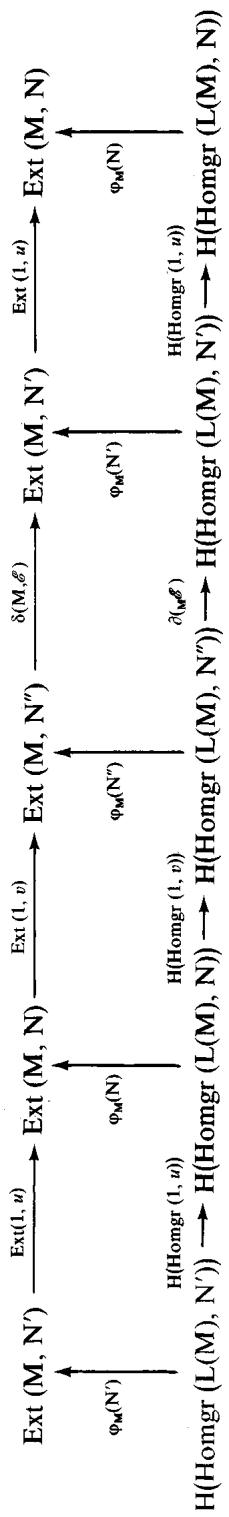
\includegraphics[keepaspectratio]{images/part001_97747f10.jpg}}

a commutative diagram of A-modules with exact rows. The diagram of k-modules

\[
\begin{array}{c} \operatorname{Ext} _ {\mathbf {A}} (\mathbf {M}, \mathbf {N} ^ {\prime \prime}) \xrightarrow {\delta (\mathbf {M} , \mathcal {E})} \operatorname{Ext} _ {\mathbf {A}} (\mathbf {M}, \mathbf {N} ^ {\prime}) \\ \operatorname{Ext} (f, g ^ {\prime \prime}) \Big | _ {\downarrow} \qquad \qquad \qquad \qquad \qquad \qquad \qquad \qquad \qquad \qquad \qquad \qquad \qquad \qquad \qquad \qquad \qquad \qquad \qquad \qquad \qquad \qquad \qquad \qquad \qquad \qquad \qquad \qquad \qquad \qquad \qquad \qquad \qquad \qquad \\ \operatorname{Ext} _ {\mathbf {A}} (\mathbf {M} _ {1}, \mathbf {N} _ {1} ^ {\prime \prime}) \xrightarrow {\delta (\mathbf {M} , \mathcal {E} _ {1})} \operatorname{Ext} _ {\mathbf {A}} (\mathbf {M} _ {1}, \mathbf {N} _ {1} ^ {\prime}) \end{array}
\]

is commutative.

This follows from X, p. 31, prop. 2 applied to the commutative diagram.

\[
\begin{array}{l} 0 \xrightarrow {\operatorname{Homgr} _ {A} (L (M) , N ^ {\prime})} \xrightarrow {\operatorname{Homgr} _ {A} (L (M) , N)} \xrightarrow {\operatorname{Homgr} _ {A} (L (M) , N ^ {\prime \prime})} 0 \\ \operatorname{Homgr} (L (f), g ^ {\prime}) \Big | _ {\downarrow} \quad \operatorname{Homgr} (1, u ^ {\prime}) \quad \Big | _ {\downarrow} \quad \operatorname{Homgr} (L (f), g) \quad \Big | _ {\downarrow} \quad \operatorname{Homgr} (L (f), g ^ {\prime \prime}) \\ 0 \xrightarrow {\operatorname{Homgr} _ {A} (L (M _ {1}) , N _ {1} ^ {\prime})} \xrightarrow {\operatorname{Homgr} _ {A} (L (M _ {1}) , N _ {1})} \xrightarrow {\operatorname{Homgr} _ {A} (L (M _ {1}) , N _ {1} ^ {\prime \prime})} 0 \end{array}
\]

Let N be an A-module, and

\[
0 \rightarrow \mathbf {M} ^ {\prime} \xrightarrow {r} \mathbf {M} \xrightarrow {s} \mathbf {M} ^ {\prime \prime} \rightarrow 0\tag{$(\mathcal{F})$}
\]

an exact sequence of A-modules; the sequence of complexes

\[
\begin{array}{r l} (\mathcal {F} _ {\mathrm{N}}) & 0 \longrightarrow \operatorname{Homgr} _ {\mathrm{A}} (\mathrm{M} ^ {\prime \prime}, \mathrm{I} (\mathrm{N})) \xrightarrow {\operatorname{Homgr} (s , 1)} \operatorname{Homgr} _ {\mathrm{A}} (\mathrm{M}, \mathrm{I} (\mathrm{N})) \\ & \xrightarrow {\operatorname{Homgr} (r , 1)} \operatorname{Homgr} _ {\mathrm{A}} (\mathrm{M} ^ {\prime}, \mathrm{I} (\mathrm{N})) \longrightarrow 0 \end{array}
\]

is exact (X, p. 83, prop. 2, a)); let

\[
\partial (\mathcal {F} _ {\mathrm{N}}): \mathrm{H} (\operatorname{Homgr} _ {\mathrm{A}} (\mathrm{M} ^ {\prime}, \mathrm{I} (\mathrm{N}))) \rightarrow \mathrm{H} (\operatorname{Homgr} _ {\mathrm{A}} (\mathrm{M} ^ {\prime \prime}, \mathrm{I} (\mathrm{N})))
\]

the corresponding connecting homomorphism.

DEFINITION 3. --- One calls connecting homomorphism of extension modules relative to the exact sequence (\(\mathcal{F}\)) and to the module N, the composite homomorphism

\[
\delta (\mathcal {F}, \mathrm{N}): \overline {{\varphi}} _ {\mathrm{N}} (\mathrm{M} ^ {\prime \prime}) \circ \partial (\mathcal {F} _ {\mathrm{N}}) \circ \overline {{\varphi}} _ {\mathrm{N}} (\mathrm{M} ^ {\prime}) ^ {- 1}: \operatorname{Ext} _ {\mathrm{A}} (\mathrm{M} ^ {\prime}, \mathrm{N}) \rightarrow \operatorname{Ext} _ {\mathrm{A}} (\mathrm{M} ^ {\prime \prime}, \mathrm{N}).
\]

This is a \(k\) -graded homomorphism of ascending degree 1, whose homogeneous components are denoted \(\delta^{n}(\mathcal{F}, \mathbf{N}) : \operatorname{Ext}_{\mathbf{A}}^{n}(\mathbf{M}', \mathbf{N}) \to \operatorname{Ext}_{\mathbf{A}}^{n+1}(\mathbf{M}'', \mathbf{N})\) .

We then prove, as above, the following statements:

THEOREM 2. --- The right-unbounded sequence of homomorphisms of k-modules

\[
\begin{array}{r l} 0 & \xrightarrow {\quad} \operatorname{Hom} _ {A} (M ^ {\prime \prime}, N) \xrightarrow {\operatorname{Hom} (s , 1)} \operatorname{Hom} _ {A} (M, N) \xrightarrow {\operatorname{Hom} (r , 1)} \operatorname{Hom} _ {A} (M ^ {\prime}, N) \\ & \xrightarrow {\delta^ {\circ} (\mathcal {F} , N)} \operatorname{Ext} _ {A} ^ {1} (M ^ {\prime \prime}, N) \to \dots \xrightarrow {\delta^ {n - 1} (\mathcal {F} , N)} \operatorname{Ext} _ {A} ^ {n} (M ^ {\prime \prime}, N) \xrightarrow {\operatorname{Ext} ^ {n} (s , 1)} \operatorname{Ext} _ {A} ^ {n} (M, N) \\ & \xrightarrow {\operatorname{Ext} ^ {n} (r , 1)} \operatorname{Ext} _ {A} ^ {n} (M ^ {\prime}, N) \xrightarrow {\delta^ {n} (\mathcal {F} , N)} \operatorname{Ext} _ {A} ^ {n + 1} (M ^ {\prime \prime}, N) \to \dots \end{array}
\]

is exact.

COROLLARY. --- If Ext \(_{A}^{1}\) (M'', N) = 0, the sequence

\[
0 \longrightarrow \operatorname{Hom} _ {\mathrm{A}} \left(\mathrm{M} ^ {\prime \prime}, \mathrm{N}\right) \xrightarrow {\operatorname{Hom} (s , 1)} \operatorname{Hom} _ {\mathrm{A}} (\mathrm{M}, \mathrm{N}) \xrightarrow {\operatorname{Hom} (r , 1)} \operatorname{Hom} _ {\mathrm{A}} \left(\mathrm{M} ^ {\prime}, \mathrm{N}\right) \longrightarrow 0
\]

is exact.

PROPOSITION 9. --- Let \(g: \mathbf{N} \to \mathbf{N}_1\) be a homomorphism of A-modules and

\[
(\mathcal {F} _ {1})
\]

\[
0 \longrightarrow \mathbf {M} _ {1} ^ {\prime} \xrightarrow {r _ {1}} \mathbf {M} _ {1} \xrightarrow {s _ {1}} \mathbf {M} _ {1} ^ {\prime \prime} \longrightarrow 0
\]

\[
f ^ {\prime} \Big \downarrow \qquad f \Big \downarrow \qquad f ^ {\prime \prime} \Big \downarrow
\]

\[
0 \longrightarrow \mathbf {M} ^ {\prime} \stackrel {r} {\longrightarrow} \mathbf {M} \stackrel {s} {\longrightarrow} \mathbf {M} ^ {\prime \prime} \longrightarrow 0\tag{$(\mathcal{F})$}
\]

a commutative diagram of A-modules with exact rows. The diagram of k-modules

\[
\begin{array}{c} \operatorname{Ext} _ {\mathbf {A}} (\mathbf {M} ^ {\prime}, \mathbf {N}) \xrightarrow {\delta (\mathcal {F} , \mathbf {N})} \operatorname{Ext} _ {\mathbf {A}} (\mathbf {M} ^ {\prime \prime}, \mathbf {N}) \\ \operatorname{Ext} _ {\mathbf {A}} (f ^ {\prime}, g) \Big \downarrow \\ \operatorname{Ext} _ {\mathbf {A}} (\mathbf {M} _ {1} ^ {\prime}, \mathbf {N} _ {1}) \xrightarrow {\delta (\mathcal {F} _ {1} , \mathbf {N} _ {1})} \operatorname{Ext} _ {\mathbf {A}} (\mathbf {M} _ {1} ^ {\prime \prime}, \mathbf {N} _ {1}) \end{array}
\]

is commutative.

\subsection{Projective modules, injective modules, and extension modules}

PROPOSITION 10. --- Let M be an A-module. The following conditions are equivalent:

\begin{enumerate}
\def\labelenumi{(\roman{enumi})}
\item
  M is projective.
\item
  \(\operatorname{Ext}_{\mathbf{A}}^{i}(\mathbf{M},\mathbf{N}) = 0\) for every A-module \(\mathbf{N}\) and for every integer \(i > 0\) .
\item
  \(\mathrm{Ext}_{\mathbf{A}}^{1}(\mathbf{M},\mathbf{N}) = 0\) for every A-module \(\mathbf{N}\) .
\item
  There exists an exact sequence
\end{enumerate}

\[
0 \rightarrow \mathrm{K} \xrightarrow {u} \mathrm{P} \xrightarrow {r} \mathrm{M} \rightarrow 0,
\]

\(\text{where P is projective, and where } \text{ Ext}_{\mathbf{A}}^{1}(\mathbf{M}, \mathbf{K}) = 0.\)

\begin{enumerate}
\def\labelenumi{(\roman{enumi})}
\item
  \(\Rightarrow\) (ii): this is the corollary of prop. 5 of X, p. 88.
\item
  \(\Rightarrow\) (iii): this is trivial.
\item
  \(\Rightarrow\) (iv): this is clear since M is a quotient of a free module P.
\item
  \(\Rightarrow\) (i): since \(\operatorname{Ext}_{\mathbf{A}}^{1}(\mathbf{M},\mathbf{K}) = 0\) the canonical map
\end{enumerate}

\[
\operatorname{Hom} _ {\mathbf {A}} (\mathbf {M}, \mathbf {P}) \rightarrow \operatorname{Hom} _ {\mathbf {A}} (\mathbf {M}, \mathbf {M})
\]

is surjective (X, p. 90, corollary); there therefore exists an A-linear section of v and M is isomorphic to a direct factor of P, hence is projective.

PROPOSITION 11. --- Let N be an A-module. The following conditions are equivalent:

\begin{enumerate}
\def\labelenumi{(\roman{enumi})}
\item
  N is injective.
\item
  \(\operatorname{Ext}_{\mathbf{A}}^{i}(\mathbf{M},\mathbf{N}) = 0\) for every A-module M and every integer \(i > 0\) .
\item
  \(\operatorname{Ext}_{\mathbf{A}}^{1}(\mathbf{M},\mathbf{N}) = 0\) for every A-module \(\mathbf{M}\) .
\item
  There exists an exact sequence
\end{enumerate}

\[
0 \rightarrow \mathrm{N} \xrightarrow {u} \mathrm{I} \xrightarrow {v} \mathrm{C} \rightarrow 0,
\]

\(\text{where I is injective and where } \text{ Ext}_{\mathbf{A}}^{1} (\mathbf{C}, \mathbf{N}) = 0;\)

\begin{enumerate}
\def\labelenumi{(\alph{enumi})}
\setcounter{enumi}{21}
\item
  \(\operatorname{Ext}_{\mathbf{A}}^{1}(\mathbf{M},\mathbf{N}) = 0\) for every monogenic A-module \(\mathbf{M}\) .
\item
  \(\Rightarrow\) (ii): this is the corollary of prop. 5 of X, p. 88.
\end{enumerate}

\begin{enumerate}
\def\labelenumi{(\roman{enumi})}
\setcounter{enumi}{1}
\item
  \(\Rightarrow\) (iii) \(\Rightarrow\) (v): this is trivial.
\item
  \(\Rightarrow\) (iv): this is clear since N is a submodule of an injective module (X, p. 19, cor. 3).
\item
  \(\Rightarrow\) (i): since \(\operatorname{Ext}_{\mathbf{A}}^{1}(\mathbf{C},\mathbf{N}) = 0\) , the canonical homomorphism
\end{enumerate}

\[
\operatorname{Hom} _ {\mathbf {A}} (\mathrm{I}, \mathbf {N}) \rightarrow \operatorname{Hom} _ {\mathbf {A}} (\mathbf {N}, \mathbf {N})
\]

is surjective (X, p. 93, corollary); there therefore exists an A-linear retraction of u and N is isomorphic to a direct factor of I, hence is injective (X, p. 16, prop. 9).

\begin{enumerate}
\def\labelenumi{(\alph{enumi})}
\setcounter{enumi}{21}
\tightlist
\item
  \(\Rightarrow\) (i): if a is an ideal of A, one has \(\operatorname{Ext}_{\mathbf{A}}^{1}(\mathbf{A}/\mathfrak{a},\mathbf{N})=0\) ; the canonical map \(\operatorname{Hom}_{\mathbf{A}}(\mathbf{A},\mathbf{N})\to\operatorname{Hom}_{\mathbf{A}}(\mathfrak{a},\mathbf{N})\) is therefore surjective and N is injective (X, p. 16, prop. 10).
\end{enumerate}

\subsection{Universal coefficient formula}

In this section, we consider two complexes of A-modules (C, d) and (C', d'). Consider the canonical exact sequences:

\[
0 \rightarrow \mathrm{Z} (\mathrm{C}) \stackrel {{j}} {{\rightarrow}} \mathrm{C} \stackrel {{\delta}} {{\rightarrow}} \mathrm{B} (\mathrm{C}) (- 1) \rightarrow 0,\tag{I}
\]

\((\mathrm{II}_{p})\)

\[
0 \to \mathrm{B} _ {p} (\mathrm{C}) \stackrel {{i}} {{\to}} \mathrm{Z} _ {p} (\mathrm{C}) \stackrel {{p}} {{\to}} \mathrm{H} _ {p} (\mathrm{C}) \to 0;
\]

we deduce from δ a k-homomorphism

\[
\mathrm{H} (\text { Homgr } (\delta , 1)): \mathrm{H} (\text { Homgr } _ {\mathbf {A}} (\mathrm{B} (\mathbf {C}), \mathbf {C} ^ {\prime})) (1) \rightarrow \mathrm{H} (\text { Homgr } _ {\mathbf {A}} (\mathbf {C}, \mathbf {C} ^ {\prime}));
\]

one deduces from \((\mathrm{II}_{p})\) connecting homomorphisms:

\[
\delta \left(\mathrm{II} _ {p}, \mathrm{H} ^ {q} \left(\mathrm{C} ^ {\prime}\right)\right): \operatorname{Hom} _ {\mathrm{A}} \left(\mathrm{B} _ {p} (\mathrm{C}), \mathrm{H} ^ {q} \left(\mathrm{C} ^ {\prime}\right)\right)\rightarrow \operatorname{Ext} _ {\mathrm{A}} ^ {1} \left(\mathrm{H} _ {p} (\mathrm{C}), \mathrm{H} ^ {q} \left(\mathrm{C} ^ {\prime}\right)\right).
\]

whence, by passing to the product, homomorphisms of k-modules

\[
\varphi^ {n}: \operatorname{Homgr} _ {\mathbf {A}} ^ {n} (\mathrm{B} (\mathrm{C}), \mathrm{H} (\mathrm{C} ^ {\prime})) \rightarrow \prod_ {p + q = n} \operatorname{Ext} _ {\mathbf {A}} ^ {1} \left(\mathrm{H} _ {p} (\mathrm{C}), \mathrm{H} ^ {q} (\mathrm{C} ^ {\prime})\right)
\]

One also has canonical homomorphisms (X, p. 82)

\[
\lambda^ {n} (\mathrm{B} (\mathrm{C}), \mathrm{C} ^ {\prime}): \mathrm{H} ^ {n} \left(\operatorname{Homgr} _ {\mathrm{A}} (\mathrm{B} (\mathrm{C}), \mathrm{C} ^ {\prime})\right)\rightarrow \operatorname{Homgr} _ {\mathrm{A}} ^ {n} (\mathrm{B} (\mathrm{C}), \mathrm{H} (\mathrm{C} ^ {\prime})) .
\]

With these notations:

THEOREM 3. --- Suppose the A-modules B(C) and Z(C) are projective. There exists, for each n, a unique homomorphism of k-modules

\[
\beta^ {n}: \prod_ {p + q = n - 1} \operatorname{Ext} _ {\mathbf {A}} ^ {1} \left(\mathrm{H} _ {p} (\mathbf {C}), \mathrm{H} ^ {q} \left(\mathbf {C} ^ {\prime}\right)\right)\rightarrow \mathrm{H} ^ {n} \left(\operatorname{Homgr} _ {\mathbf {A}} \left(\mathrm{C}, \mathrm{C} ^ {\prime}\right)\right)
\]

thereby making the diagram commutative

\[
\begin{array}{c} \operatorname{Homgr} _ {\mathbf {A}} ^ {n - 1} (\mathrm{B} (\mathrm{C}), \mathrm{H} (\mathrm{C} ^ {\prime})) \xleftarrow {\lambda^ {n - 1} (\mathrm{B} (\mathrm{C}) , \mathrm{C} ^ {\prime})} \mathrm{H} ^ {n - 1} (\operatorname{Homgr} _ {\mathbf {A}} (\mathrm{B} (\mathrm{C}), \mathrm{C} ^ {\prime})) \\ \prod_ {p + q = n - 1} \operatorname{Ext} _ {\mathbf {A}} ^ {1} (\mathrm{H} _ {p} (\mathrm{C}), \mathrm{H} ^ {q} (\dot {\mathrm{C}} ^ {\prime})) \xrightarrow {\beta^ {n}} \mathrm{H} ^ {n} (\operatorname{Homgr} _ {\mathbf {A}} (\mathrm{C}, \mathrm{C} ^ {\prime})). \end{array}
\]

The sequences of graded k-modules

\[
\begin{array}{r l} 0 \longrightarrow & \prod_ {p + q = n - 1} \operatorname{Ext} _ {\mathrm{A}} ^ {1} \left(\mathrm{H} _ {p} (\mathrm{C}), \mathrm{H} ^ {q} (\mathrm{C} ^ {\prime})\right) \xrightarrow {\beta^ {n}} \mathrm{H} ^ {n} \big (\mathrm{Homg} _ {\mathrm{A}} (\mathrm{C}, \mathrm{C} ^ {\prime}) \big) \\ & \xrightarrow {\lambda^ {n} (\mathrm{C} , \mathrm{C} ^ {\prime})} \prod_ {p + q = n} \mathrm{Hom} _ {\mathrm{A}} \left(\mathrm{H} _ {p} (\mathrm{C}), \mathrm{H} ^ {q} (\mathrm{C} ^ {\prime})\right) \to 0 \end{array}\tag{11}
\]

are exact.

Remark. --- One can prove an analogous statement, assuming \(\mathbf{B}_{n}(\mathbf{C}')\) and \(\mathbf{C}'/\mathbf{B}_{n}(\mathbf{C}')\) injective for each n.

For simplicity set \(\mathbf{B} = \mathbf{B}(\mathbf{C}), \mathbf{Z} = \mathbf{Z}(\mathbf{C}), \mathbf{H} = \mathbf{H}(\mathbf{C})\) and \(\mathbf{H}' = \mathbf{H}(\mathbf{C}')\) . Since B is projective, from (I) one derives an exact sequence

\[
\begin{array}{r l}(1 2) \quad&0 \rightarrow \operatorname{Homgr} _ {\mathbf {A}} (\mathrm{B}, \mathrm{C} ^ {\prime}) (1) \xrightarrow {\operatorname{Homgr} (\delta , 1)} \operatorname{Homgr} _ {\mathbf {A}} (\mathrm{C}, \mathrm{C} ^ {\prime})\\&\xrightarrow {\operatorname{Homgr} (j , 1)} \operatorname{Homgr} _ {\mathbf {A}} (\mathrm{Z}, \mathrm{C} ^ {\prime}) \rightarrow 0.\end{array}
\]

Lemma 2. --- The connecting homomorphism

\[
\mathrm{H} ^ {n} \left(\operatorname{Homgr} _ {\mathbf {A}} \left(\mathrm{Z}, \mathrm{C} ^ {\prime}\right)\right)\rightarrow \mathrm{H} ^ {n} \left(\operatorname{Homgr} _ {\mathbf {A}} \left(\mathrm{B}, \mathrm{C} ^ {\prime}\right)\right)
\]

associated with (12) is equal to \((-1)^{n+1}\) H(Homgr(i, 1)).

Indeed, let \(a \in \mathbf{Z}^n(\text{Homgr}_A(Z, C'))\) ; this is a morphism of complexes of ascending degree \(n\) of \(Z\) to \(C'\) , whose values therefore lie in \(Z(C')\) . Since the exact sequence (I) is split (B being projective), \(a\) extends to an element \(b\) of \(\text{Homgr}_A^n(C, Z(C'))\) . By definition, the image of the class of \(a\) under the connecting homomorphism in question is the class in \(H^n(\text{Homgr}_A(B, C'))\) of the homomorphism \(u\) of \(B(C)\) to \(C'\) such that for \(x \in C\) , one has

\[
u (d x) = \mathrm{D} b (x) = d ^ {\prime} b (x) - (- 1) ^ {n} b (d x) = (- 1) ^ {n + 1} b (d x) = (- 1) ^ {n + 1} a (d x),
\]

whence the assertion.

The exact homology sequence associated with (12) therefore gives the exact sequence

\[
\rightarrow \mathrm{H} ^ {n} (\operatorname{Homgr} _ {\mathrm{A}} (Z, C ^ {\prime})) \xrightarrow {\mathrm{H} (\operatorname{Homgr} (i , 1))} \mathrm{H} ^ {n} (\operatorname{Homgr} _ {\mathrm{A}} (B, C ^ {\prime}))
\]

\[
\xrightarrow {\mathrm{H} (\text { Homgr } (\delta , 1))} \mathrm{H} ^ {n + 1} \left(\text { Homgr } _ {\mathrm{A}} \left(\mathrm{C}, \mathrm{C} ^ {\prime}\right)\right) \xrightarrow {\mathrm{H} (\text { Homgr } (j , 1))} \mathrm{H} ^ {n + 1} \left(\text { Homgr } _ {\mathrm{A}} \left(\mathrm{Z}, \mathrm{C} ^ {\prime}\right)\right)\rightarrow \dots .
\]

Moreover, since Z is projective, one derives from \((II_{p})\) exact sequences

\[
0 \to \mathrm{Hom} _ {\mathbf {A}} (\mathrm{H} _ {p}, \mathrm{H} ^ {\prime q}) \to \mathrm{Hom} _ {\mathbf {A}} (Z _ {p}, \mathrm{H} ^ {\prime q}) \to \mathrm{Hom} _ {\mathbf {A}} (\mathrm{B} _ {p}, \mathrm{H} ^ {\prime q}) \to \mathrm{Ext} _ {\mathbf {A}} ^ {1} (\mathrm{H} _ {p}, \mathrm{H} ^ {\prime q}) \to 0,
\]

whence, by passing to products, exact sequences

\[
\begin{array}{r l} 0 \to \operatorname{Homgr} _ {\mathbf {A}} ^ {n} (\mathbf {H}, \mathbf {H} ^ {\prime}) & \to \operatorname{Homgr} _ {\mathbf {A}} ^ {n} (Z, \mathbf {H} ^ {\prime}) \to \operatorname{Homgr} _ {\mathbf {A}} ^ {n} (\mathbf {B}, \mathbf {H} ^ {\prime}) \\ & \to \prod_ {p + q = n} \operatorname{Ext} _ {\mathbf {A}} ^ {1} (\mathbf {H} _ {p}, \mathbf {H} ^ {\prime q}) \to 0. \end{array}
\]

Finally, one has the canonical homomorphisms of no. 1:

\[
\begin{array}{l} \lambda_ {\mathrm{B}} = \lambda (\mathrm{B}, \mathrm{C} ^ {\prime}): \mathrm{H} (\mathrm{Homgr} _ {\mathrm{A}} (\mathrm{B}, \mathrm{C} ^ {\prime})) \to \mathrm{Homgr} _ {\mathrm{A}} (\mathrm{B}, \mathrm{H} ^ {\prime}), \\ \lambda_ {\mathrm{Z}} = \lambda (\mathrm{Z}, \mathrm{C} ^ {\prime}): \mathrm{H} (\mathrm{Homgr} _ {\mathrm{A}} (\mathrm{Z}, \mathrm{C} ^ {\prime})) \to \mathrm{Homgr} _ {\mathrm{A}} (\mathrm{Z}, \mathrm{H} ^ {\prime}), \\ \lambda_ {\mathrm{C}} = \lambda (\mathrm{C}, \mathrm{C} ^ {\prime}): \mathrm{H} (\mathrm{Homgr} _ {\mathrm{A}} (\mathrm{C}, \mathrm{C} ^ {\prime})) \to \mathrm{Homgr} _ {\mathrm{A}} (\mathrm{H}, \mathrm{H} ^ {\prime}), \end{array}
\]

whence the diagram with exact rows on page X. 97.

This diagram is commutative by construction of the homomorphisms \(\lambda\) . Moreover, since the complexes B and Z are split and projective, \(\lambda_{\mathrm{B}}\) and \(\lambda_{\mathrm{Z}}\) are bijective (X, p. 84, cor. 1). From this one deduces, on the one hand, that \(\lambda_{\mathrm{C}}^{n}\) is surjective, with kernel equal to Im H \(^{n}\) (Homgr ( \(\delta\) , 1)), and on the other hand, that \(\varphi^{n-1} \circ \lambda_{\mathrm{B}}^{n-1}\) is surjective, with kernel equal to Ker H \(^{n}\) (Homgr ( \(\delta\) , 1)). The theorem follows immediately from this.

COROLLARY 1. --- Suppose B(C) and Z(C) are projective and B \(^{n}\) (C') is injective for each n. Then the exact sequences (11) are split.

This follows from the theorem and the following lemma:

Lemma 3. --- If B(C) is projective and \(\mathbf{B}_{n}(\mathbf{C}^{\prime})\) injective for each \(n\) , the canonical homomorphism \(\lambda(\mathbf{C}, \mathbf{C}^{\prime}): \mathrm{H}(\mathrm{Homgr}_{\mathbf{A}}(\mathbf{C}, \mathbf{C}^{\prime})) \to \mathrm{Homgr}_{\mathbf{A}}(\mathrm{H}(\mathbf{C}), \mathrm{H}(\mathbf{C}^{\prime}))\) has a section \(k\) -linear.

Indeed, according to X, p. 35, remarks a) and b), there exist homologisms

\[
\varphi : \mathrm{C} \rightarrow \mathrm{H} (\mathrm{C}) \quad \text { and } \quad \varphi^ {\prime}: \mathrm{H} (\mathrm{C} ^ {\prime}) \rightarrow \mathrm{C} ^ {\prime}
\]

such that \(\mathbf{H}(\varphi) = 1_{\mathbf{H}(\mathbf{C})}\) and \(\bar{\mathbf{H}} (\varphi^{\prime}) = 1_{\mathbf{H}(\mathbf{C}^{\prime})}\) .

In the commutative diagram

\[
\begin{array}{l} \mathrm{H} (\operatorname{Homgr} _ {\mathbf {A}} (\mathrm{H} (\mathrm{C}), \mathrm{H} (\mathrm{C} ^ {\prime})) \xrightarrow {\mathrm{H} (\operatorname{Homgr} (\varphi , \varphi^ {\prime}))} \mathrm{H} (\operatorname{Homgr} _ {\mathbf {A}} (\mathrm{C}, \mathrm{C} ^ {\prime})) \\ \lambda (\mathrm{H} (\mathrm{C}), \mathrm{H} (\mathrm{C} ^ {\prime})) \Big | _ {\downarrow} \\ \operatorname{Homgr} _ {\mathbf {A}} (\mathrm{H} (\mathrm{C}), \mathrm{H} (\mathrm{C} ^ {\prime})) \xrightarrow {\operatorname{Homgr} (\mathrm{H} (\varphi) , \mathrm{H} (\varphi^ {\prime}))} \operatorname{Homgr} _ {\mathbf {A}} (\mathrm{H} (\mathrm{C}), \mathrm{H} (\mathrm{C} ^ {\prime}))  , \end{array}
\]

\(\lambda(H(C), H(C'))\) is bijective and Homgr \((H(\varphi), H(\varphi'))\) is the identity, whence the assertion.

Homgr \(^{n-1}\) (Z, H') → Homgr \(^{n-1}\) (B, H') → Φ \(^{n-1}\) → Πp+q=n-1 Ext \(^{1}\) (Hp, H'q) → 0

H \(^{n-1}\) (Homgr(A, C')) → H \(^{n-1}\) (Homgr(A, B, C')) → H \(^{n}\) (Homgr(A, C)) → H \(^{n}\) (Homgr(A, C)) → H \(^{n}\) (Homgr(A, B, C))

0 → Homgr \(^{n}\) (H, H') → Homgr \(^{n}\) (Z, H') → Homgr \(^{n}\) (B, H')

COROLLARY 2. --- If B(C) and Z(C) are projective, then, for every A-module N and every integer n, there is a split exact sequence:

\[
(1 3) \quad 0 \longrightarrow \operatorname{Ext} _ {\mathbf {A}} ^ {1} \left(\mathrm{H} _ {n - 1} (\mathrm{C}), \mathrm{N}\right) \xrightarrow {\beta^ {n}} \mathrm{H} ^ {n} \left(\operatorname{Homgr} _ {\mathbf {A}} (\mathrm{C}, \mathrm{N})\right) \xrightarrow {\lambda^ {n}} \operatorname{Hom} _ {\mathbf {A}} \left(\mathrm{H} _ {n} (\mathrm{C}), \mathrm{N}\right) \longrightarrow 0.
\]

COROLLARY 3 (“universal coefficient formula”). --- Suppose A is principal and C is free. Then for every A-module N and every integer n, there is a split exact sequence (13).

Indeed, B(C) and Z(C) are free as submodules of the free module C (VII, § 3, cor. 2 to th. 1).

COROLLARY 4. --- If C is bounded on the right and if C and H(C) are projective, then

\[
\lambda (C, C ^ {\prime}): H \left(\operatorname{Homgr} _ {A} (C, C ^ {\prime})\right)\rightarrow \operatorname{Homgr} _ {A} \left(H (C), H \left(C ^ {\prime}\right)\right)
\]

is bijective.

By the theorem, it suffices to prove that B(C) and Z(C) are projective. Now we have exact sequences

\[
\begin{array}{l} 0 \to \mathrm{B} _ {n} (\mathrm{C}) \to Z _ {n} (\mathrm{C}) \to \mathrm{H} _ {n} (\mathrm{C}) \to 0 \\ 0 \to Z _ {n} (\mathrm{C}) \to \mathrm{C} _ {n} \to \mathrm{B} _ {n - 1} (\mathrm{C}) \to 0, \end{array}
\]

hence \((\mathbf{B}_{n - 1}(\mathbf{C})\) is projective) \(\Rightarrow (\mathbf{Z}_n(\mathbf{C})\) is projective) \(\Rightarrow (\mathbf{B}_n(\mathbf{C})\) is projective). We conclude by noting that \(\mathbf{B}_n(\mathbf{C}) = 0\) for \(n\) small enough.

\subsection{Generalization to complexes of multimodules; the canonical isomorphisms}

Let B, B' be two rings, C a complex of (A, B)-bimodules, C' a complex of (A, B')-bimodules; then (Homgr\_A (C, C′), D) is a complex of (B, B′)-bimodules, and the canonical homomorphism \(\lambda: H(\text{Homgr}_A (\text{C}, \text{C'})) \to \text{Homgr}_A (\text{H}(\text{C}), \text{H}(\text{C'}))\) is a homomorphism of (B, B')-bimodules.

If M is an (A, B)-bimodule and N an (A, B')-bimodule, then Homgr \(_{A}\) (L(M), I(N)) is a complex of (B, B')-bimodules, so that Ext \(_{A}\) (M, N) is endowed with a natural structure of graded (B, B')-bimodule; on the degree 0 term, this structure coincides with that of Hom \(_{A}\) (M, N) (II, p. 35).

If \(\lambda\in\mathbf{B},\lambda^{\prime}\in\mathbf{B}^{\prime}\) and if we denote \(\lambda_{\mathrm{M}},\lambda_{\mathrm{N}}^{\prime},\lambda_{\mathrm{E}},\lambda_{\mathrm{E}}^{\prime}\) the homotheties \(x\mapsto x\lambda,y\mapsto y\lambda^{\prime},z\mapsto\lambda z,z\mapsto z\lambda^{\prime}\) of M, N, Ext \(_{\mathrm{A}}\) (M, N), Ext \(_{\mathrm{A}}\) (M, N) respectively, we then have

\[
\lambda_ {\mathrm{E}} = \operatorname{Ext} _ {\mathbf {A}} \left(\lambda_ {\mathbf {M}}, 1\right), \quad \lambda_ {\mathrm{E}} ^ {\prime} = \operatorname{Ext} \left(1, \lambda_ {\mathbf {N}} ^ {\prime}\right),
\]

which provides another description of the bimodule structure of Ext \(_{A}\) (M, N). We leave it to the reader to generalize nos. 4 and 6 to the case of complexes of multimodules.

Let C, C′, and C′′ be complexes of A-modules. Composition of maps defines a graded homomorphism of degree zero:

\[
\operatorname{Homgr} _ {\mathbf {A}} \left(\mathrm{C} ^ {\prime}, \mathrm{C} ^ {\prime \prime}\right) \otimes_ {k} \operatorname{Homgr} _ {\mathbf {A}} \left(\mathrm{C}, \mathrm{C} ^ {\prime}\right)\rightarrow \operatorname{Homgr} _ {\mathbf {A}} \left(\mathrm{C}, \mathrm{C} ^ {\prime \prime}\right).\tag{14}
\]

Let B, B', E be rings, C, C', C'' of complexes of (B', A)-bimodules, (A, E)-bimodules, (B, E)-bimodules respectively. By restriction of the canonical isomorphism of II, p. 73, one obtains a bijective homomorphism of (B, B')-bimodules:

\[
\operatorname{Homgr} _ {E} \left(C \otimes_ {A} C ^ {\prime}, C ^ {\prime \prime}\right)\rightarrow \operatorname{Homgr} _ {A} \left(C, \operatorname{Homgr} _ {E} \left(C ^ {\prime}, C ^ {\prime \prime}\right)\right).\tag{15}
\]

Finally, let B be a ring, C a complex of right B-modules, C' a complex of right A-modules, C'' a complex of (B, A)-bimodules. We deduce from the canonical homomorphisms (II, p. 75)

\[
\mathrm{C} _ {p} \otimes_ {\mathrm{B}} \operatorname{Hom} _ {\mathrm{A}} \left(\mathrm{C} _ {q} ^ {\prime}, \mathrm{C} _ {r} ^ {\prime \prime}\right)\rightarrow \operatorname{Hom} _ {\mathrm{A}} \left(\mathrm{C} _ {q} ^ {\prime}, \mathrm{C} _ {p} \otimes_ {\mathrm{B}} \mathrm{C} _ {r} ^ {\prime \prime}\right)
\]

a graded homomorphism of degree zero:

\[
\mathrm{C} \otimes_ {\mathrm{B}} \operatorname{Homgr} _ {\mathrm{A}} \left(\mathrm{C} ^ {\prime}, \mathrm{C} ^ {\prime \prime}\right)\rightarrow \operatorname{Homgr} _ {\mathrm{A}} \left(\mathrm{C} ^ {\prime}, \mathrm{C} \otimes_ {\mathrm{B}} \mathrm{C} ^ {\prime \prime}\right).\tag{16}
\]

This homomorphism is bijective when C is a finitely generated projective module (II, p. 75, prop. 2).

PROPOSITION 12. --- The homomorphisms (14), (15), (16) are morphisms of complexes.

Let us prove it, for example, for the homomorphism (14). Denote

\[
\kappa : \operatorname{Homgr} _ {\mathbf {A}} \left(\mathrm{C} ^ {\prime}, \mathrm{C} ^ {\prime \prime}\right) \otimes_ {k} \operatorname{Homgr} _ {\mathbf {A}} \left(\mathrm{C}, \mathrm{C} ^ {\prime}\right)\rightarrow \operatorname{Homgr} _ {\mathbf {A}} \left(\mathrm{C}, \mathrm{C} ^ {\prime \prime}\right)
\]

this homomorphism. Let \(f \in \operatorname{Homgr}_{\mathbf{A}}(\mathbf{C}', \mathbf{C}^{\prime})_{p}\) and \(g \in \operatorname{Homgr}_{\mathbf{A}}(\mathbf{C}, \mathbf{C}^{\prime})_{q}\) ; we then have by definition \(\kappa(f \otimes g) = f \circ g\) Moreover:

\[
\begin{array}{r l} \mathrm{D} (f \otimes g) = & \mathrm{D} f \otimes g + (- 1) ^ {p} f \otimes \mathrm{D} g = (d ^ {\prime \prime} \circ f) \otimes g - (- 1) ^ {p} (f \circ d ^ {\prime}) \otimes g + \\ & + (- 1) ^ {p} f \otimes (d ^ {\prime} \circ g) - (- 1) ^ {p + q} f \otimes (g \circ d), \end{array}
\]

whence

\[
\begin{array}{r l} & {\kappa \big (\mathbf {D} (f \otimes g) \big) = d ^ {\prime \prime} \circ f \circ g - (- 1) ^ {p} f \circ d ^ {\prime} \circ g +} \\ & {\qquad + (- 1) ^ {p} f \circ d ^ {\prime} \circ g - (- 1) ^ {p + q} f \circ g \circ d} \\ & {\qquad = d ^ {\prime \prime} \circ f \circ g - (- 1) ^ {p + q} f \circ g \circ d = \mathbf {D} (f \circ g) = \mathbf {D} \big (\kappa (f \otimes g) \big).} \end{array}
\]

One proves similarly that the homomorphisms (15) and (16) are morphisms of complexes.

From the morphism (14) we deduce homomorphisms of \(k\) -modules (X, p. 62)

\[
\mathrm{H} ^ {p} \left(\operatorname{Homgr} _ {\mathbf {A}} \left(\mathrm{C} ^ {\prime}, \mathrm{C} ^ {\prime \prime}\right)\right) \otimes_ {k} \mathrm{H} ^ {q} \left(\operatorname{Homgr} _ {\mathbf {A}} \left(\mathrm{C}, \mathrm{C} ^ {\prime}\right)\right)\rightarrow \mathrm{H} ^ {p + q} \left(\operatorname{Homgr} _ {\mathbf {A}} \left(\mathrm{C}, \mathrm{C} ^ {\prime \prime}\right)\right). \tag {17}
\]

Taking C = A, we see that the homomorphism:

\[
\operatorname{Homgr} _ {\mathbf {A}} \left(\mathrm{C} ^ {\prime}, \mathrm{C} ^ {\prime \prime}\right) \otimes_ {k} \mathrm{C} ^ {\prime} \rightarrow \mathrm{C} ^ {\prime \prime}\tag{18}
\]

which maps \(f \otimes x\) to \(f(x)\) is a morphism of complexes of left A-modules; associated to it is a canonical homomorphism (X, p. 80) of graded A-modules \(\gamma : \mathrm{H}(\mathrm{Homgr}_{\mathbf{A}}(\mathbf{C}', \mathbf{C}')) \otimes_k \mathrm{H}(\mathbf{C}') \to \mathrm{H}(\mathbf{C}'')\) , which corresponds to the canonical homomorphism of \(k\) -modules

\[
\lambda : \mathrm{H} (\operatorname{Homgr} _ {\mathbf {A}} \left(\mathrm{C} ^ {\prime}, \mathrm{C} ^ {\prime \prime}\right)) \rightarrow \operatorname{Homgr} _ {\mathbf {A}} \left(\mathrm{H} (\mathrm{C} ^ {\prime}), \mathrm{H} (\mathrm{C} ^ {\prime \prime})\right).
\]

\section{USE OF NON-CANONICAL RESOLUTIONS}

We resume the conventions of § 4.
